\chapter{Materiais e Método}
\vspace{-2.5 cm}

Este Capítulo descreve os requisitos materiais para o desenvolvimento do
trabalho e os métodos que serão adotados para atingir os objetivos. 

\section{Materiais}

Os materiais a serem utilizados dividem-se em componentes eletrônicos e
componentes físicos. Os componentes eletrônicos podem ser vistos na tabela \ref{tab:custo}.

\begin{table}[ht]
\caption{Tabela de custos}
\vspace{0.2 cm}
%\footnotesize
\resizebox{\linewidth}{!}{
\begin{tabular}{ll|l|l|l}
\cline{1-4}
\multicolumn{1}{|l|}{\textbf{Item}}                                                     
& \textbf{Qtd} & \textbf{Custo Unitário} & \textbf{Custo Total} &  \\
\cline{1-4}
\multicolumn{1}{|l|}{Bateria LiPo Limskey 11,1v 3S 4200mAh}                     
& 1   & 112,05              & 112,05           &  \\ \cline{1-4}
\multicolumn{1}{|l|}{Módulo para cartão de memória SD WAVGAT, comunicação SPI}                          & 1   & 2,79           & 2,79        &  \\ \cline{1-4}
\multicolumn{1}{|l|}{Ponte H dupla L298N}                                                               & 1   & 6,12           & 6,12        &  \\ \cline{1-4}
\multicolumn{1}{|l|}{Sensor infravermelho GP2Y0A21YK0F, alcance de 10 a 80 cm}                          & 5   & 13,07          & 65,35       &  \\ \cline{1-4}
\multicolumn{1}{|l|}{Módulo conversor Buck DC-DC, saída 5v}                     
& 1   & 9,14           & 9,14        &  \\ \cline{1-4}
\multicolumn{1}{|l|}{Sensor inercial IMU GY-87, com 10 graus de liberdade (MPU6050, HCM5883L, BMP180)}  & 1   & 25,9           & 25,9        &  \\ \cline{1-4}
\multicolumn{1}{|l|}{Módulo wireless NRF24L01 com antena de alcance de 1000
metros}                     & 1   & 7,69              & 7,69           &  \\
\cline{1-4}
\multicolumn{1}{|l|}{Conjuntos de motores, caixa de redução 1:34 e sensores de efeito hall (341,2 PPR)} & 2   & 47,015         & 94,03       &  \\ \cline{1-4}
\multicolumn{1}{|l|}{Esfera de rolagem}                                                                 & 1   & 2,002          & 2,002       &  \\ \cline{1-4}
\multicolumn{1}{|l|}{Tiva Connected LaunchPad TM4C1294
}& 1   & 80,00 & 80,00 &  \\ \cline{1-4} 
                                                                                                        
                                                                                                        
                                                                                                        &
                                                                                                        &
                                                                                                        Total:
                                                                                                        &
                                                                                                        405,07     &  \\ \cline{3-4}
\end{tabular}}
\label{tab:custo}
\end{table}

Materiais para o corpo do robô, como chapa de MDF para o chassi, parafusos
de rosca, abraçadeiras não tiveram seus custos contabilizados.

Entre as ferramentas, será utilizado \textit{software} Matlab, com o
simulador Simiam \cite{Simiam}, que é implementado como um aplicativo Matlab.

\subsection{O simulador Simiam e alterações necessárias}

O Simulador Simiam foi implementado pela Universidade Georgia Tech, 
inicialmente oferecendo apenas suporte ao robô Khepera 3. Posteriormente, 
para atender necessidades do curso \textit{Control of Mobile Robots}, hospedado 
na plataforma ``Coursera.org'', o robô de baixo custo QuickBot foi adicionado. 
Os robôs Khepera e QuickBot reais podem ser vistos na Figura \ref{fig:RobosK3QB}. 
Suas contrapartes simuladas estão retratadas na Figura \ref{fig:RobosEmSimulador}.

O curso mencionado foi removido da plataforma no dia 17 de Agosto de 2020 e apenas
os alunos concluíntes possuem acesso. De qualquer forma, o simulador ainda pode ser
obtido gratuitamente.

\begin{figure}[ht]
\centering
\caption{Robôs Khepera 3 e QuickBot}
\label{fig:RobosK3QB}
	\begin{subfigure}[b]{0.49\textwidth}%
		\centering
		% fbox{}
		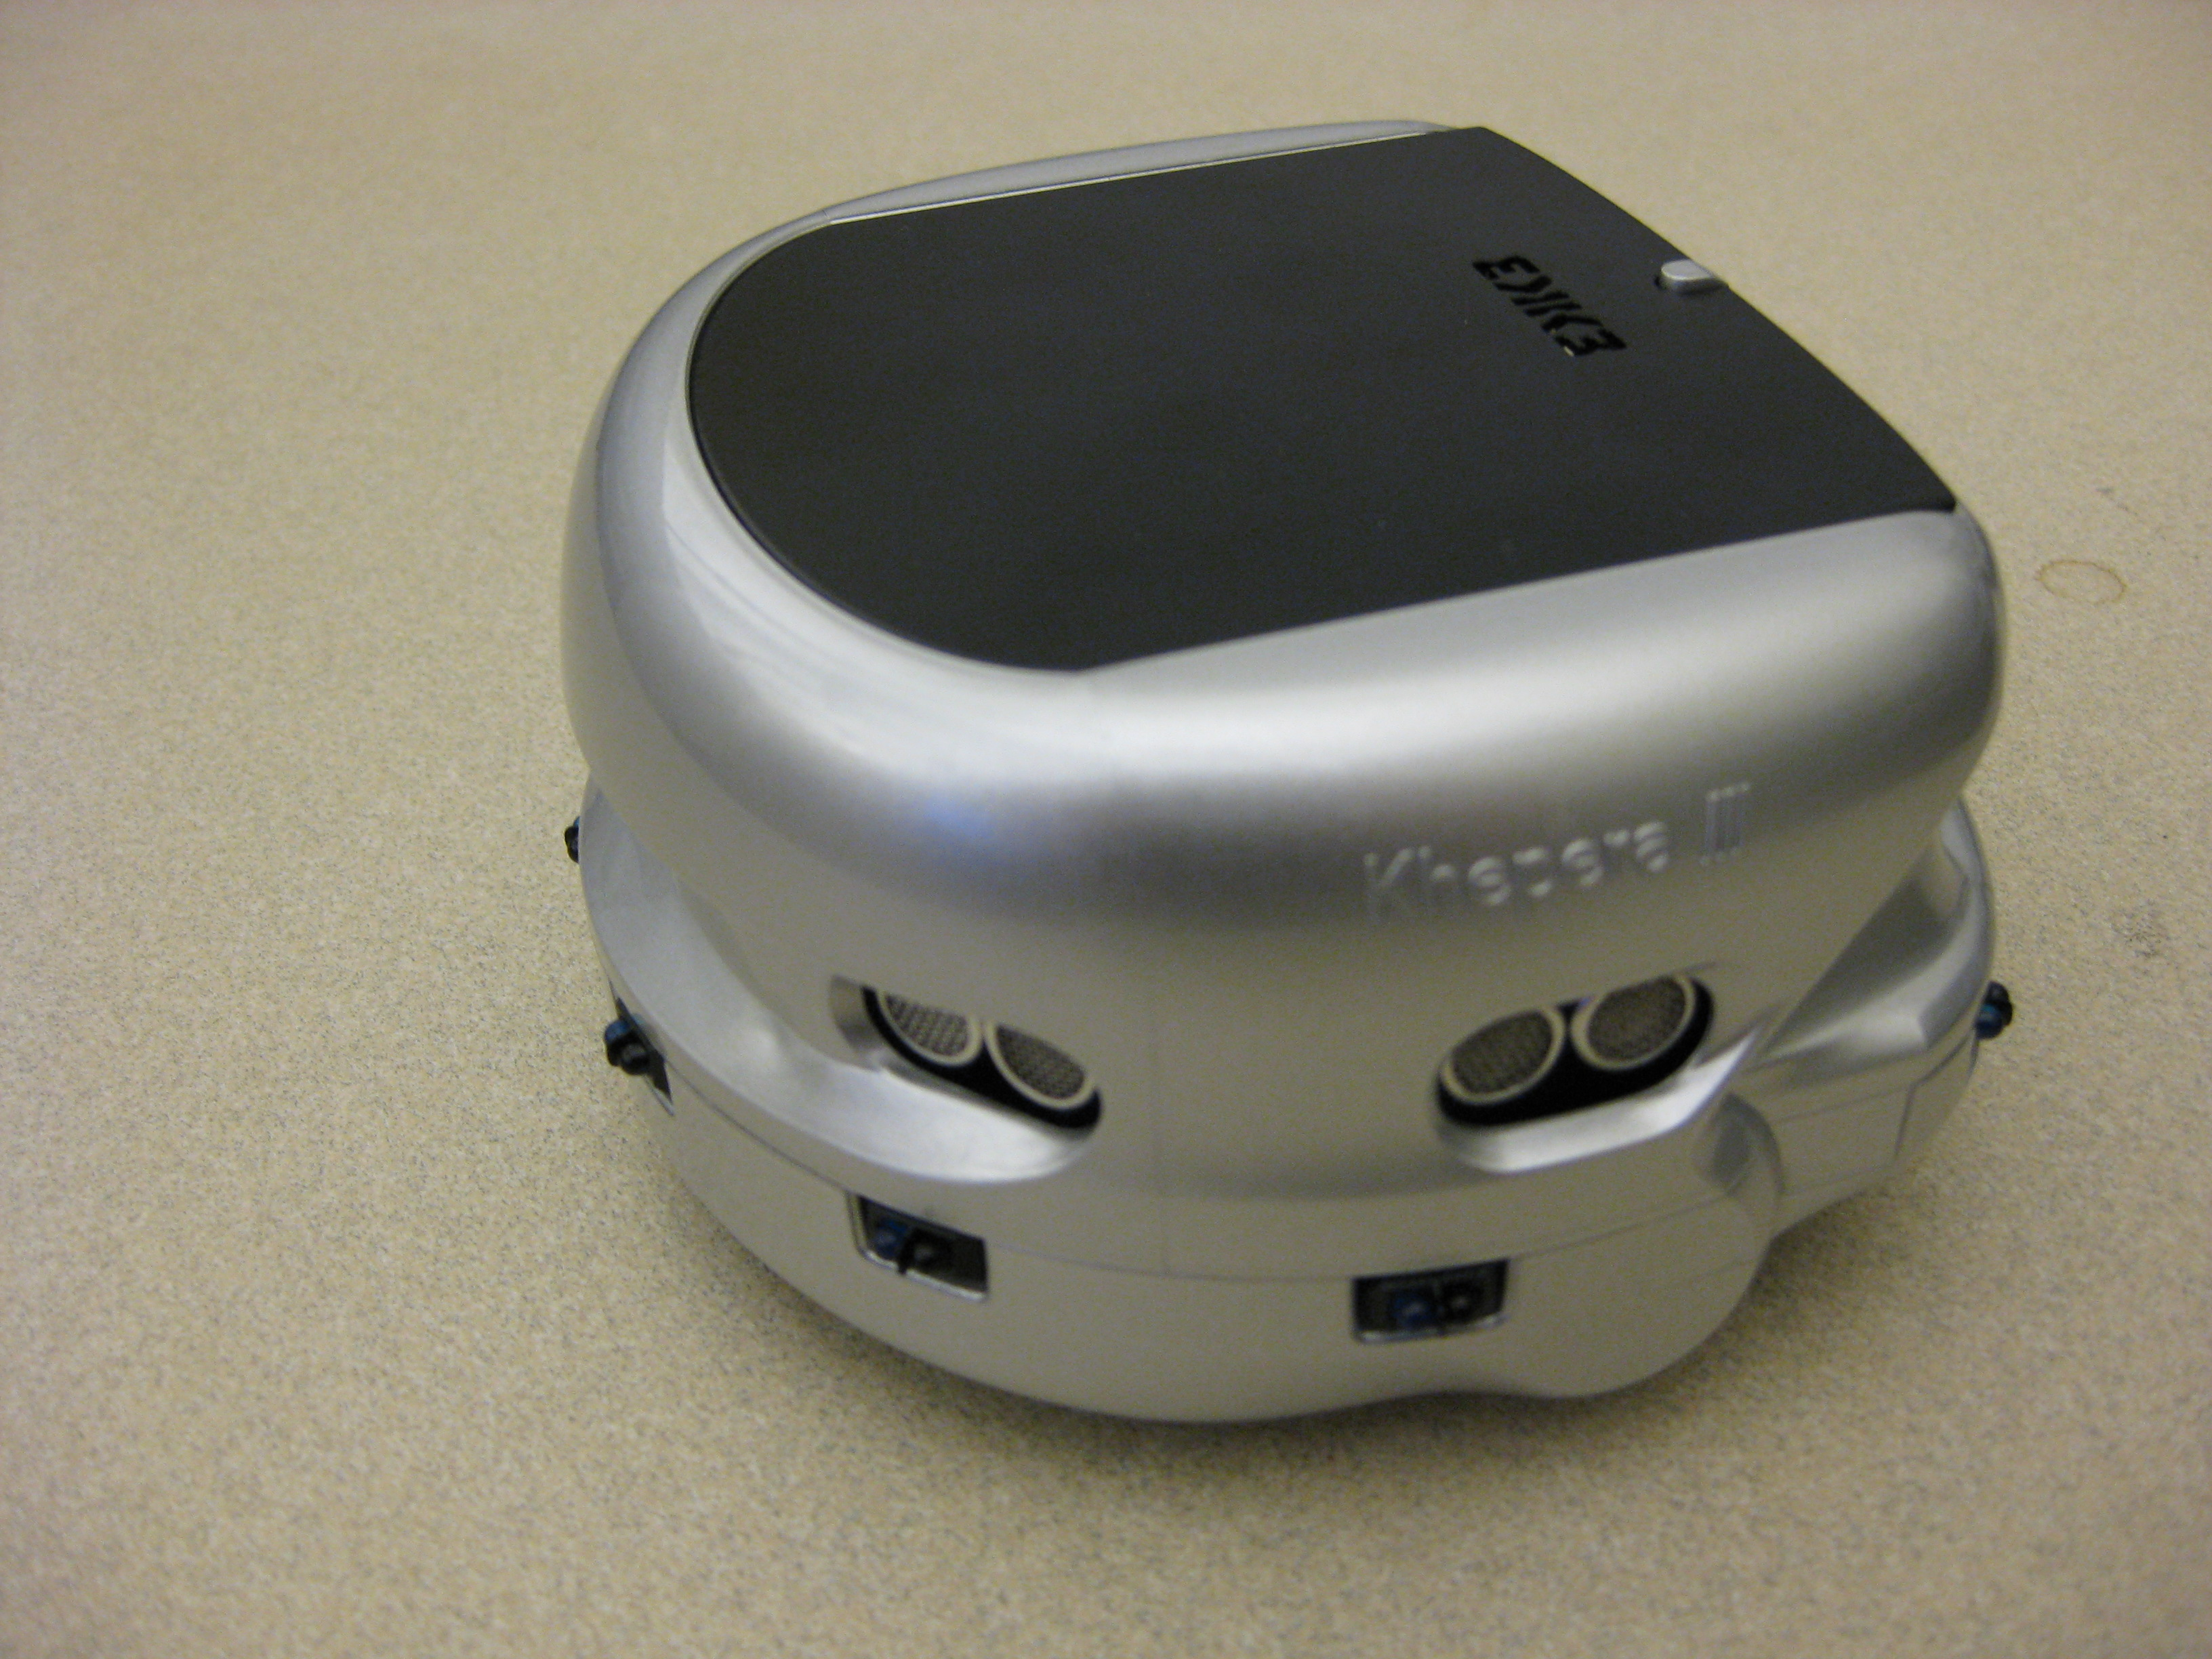
\includegraphics[trim= 8cm 0cm 0cm 0cm,clip,
scale=0.14]{Figuras/Khepera_III_robot}
		\subcaption{Robô Khepera 3}
	  	\label{fig:test1}
	\end{subfigure}
	~
	\begin{subfigure}[b]{0.49\textwidth}%
		\centering
		% fbox{}
		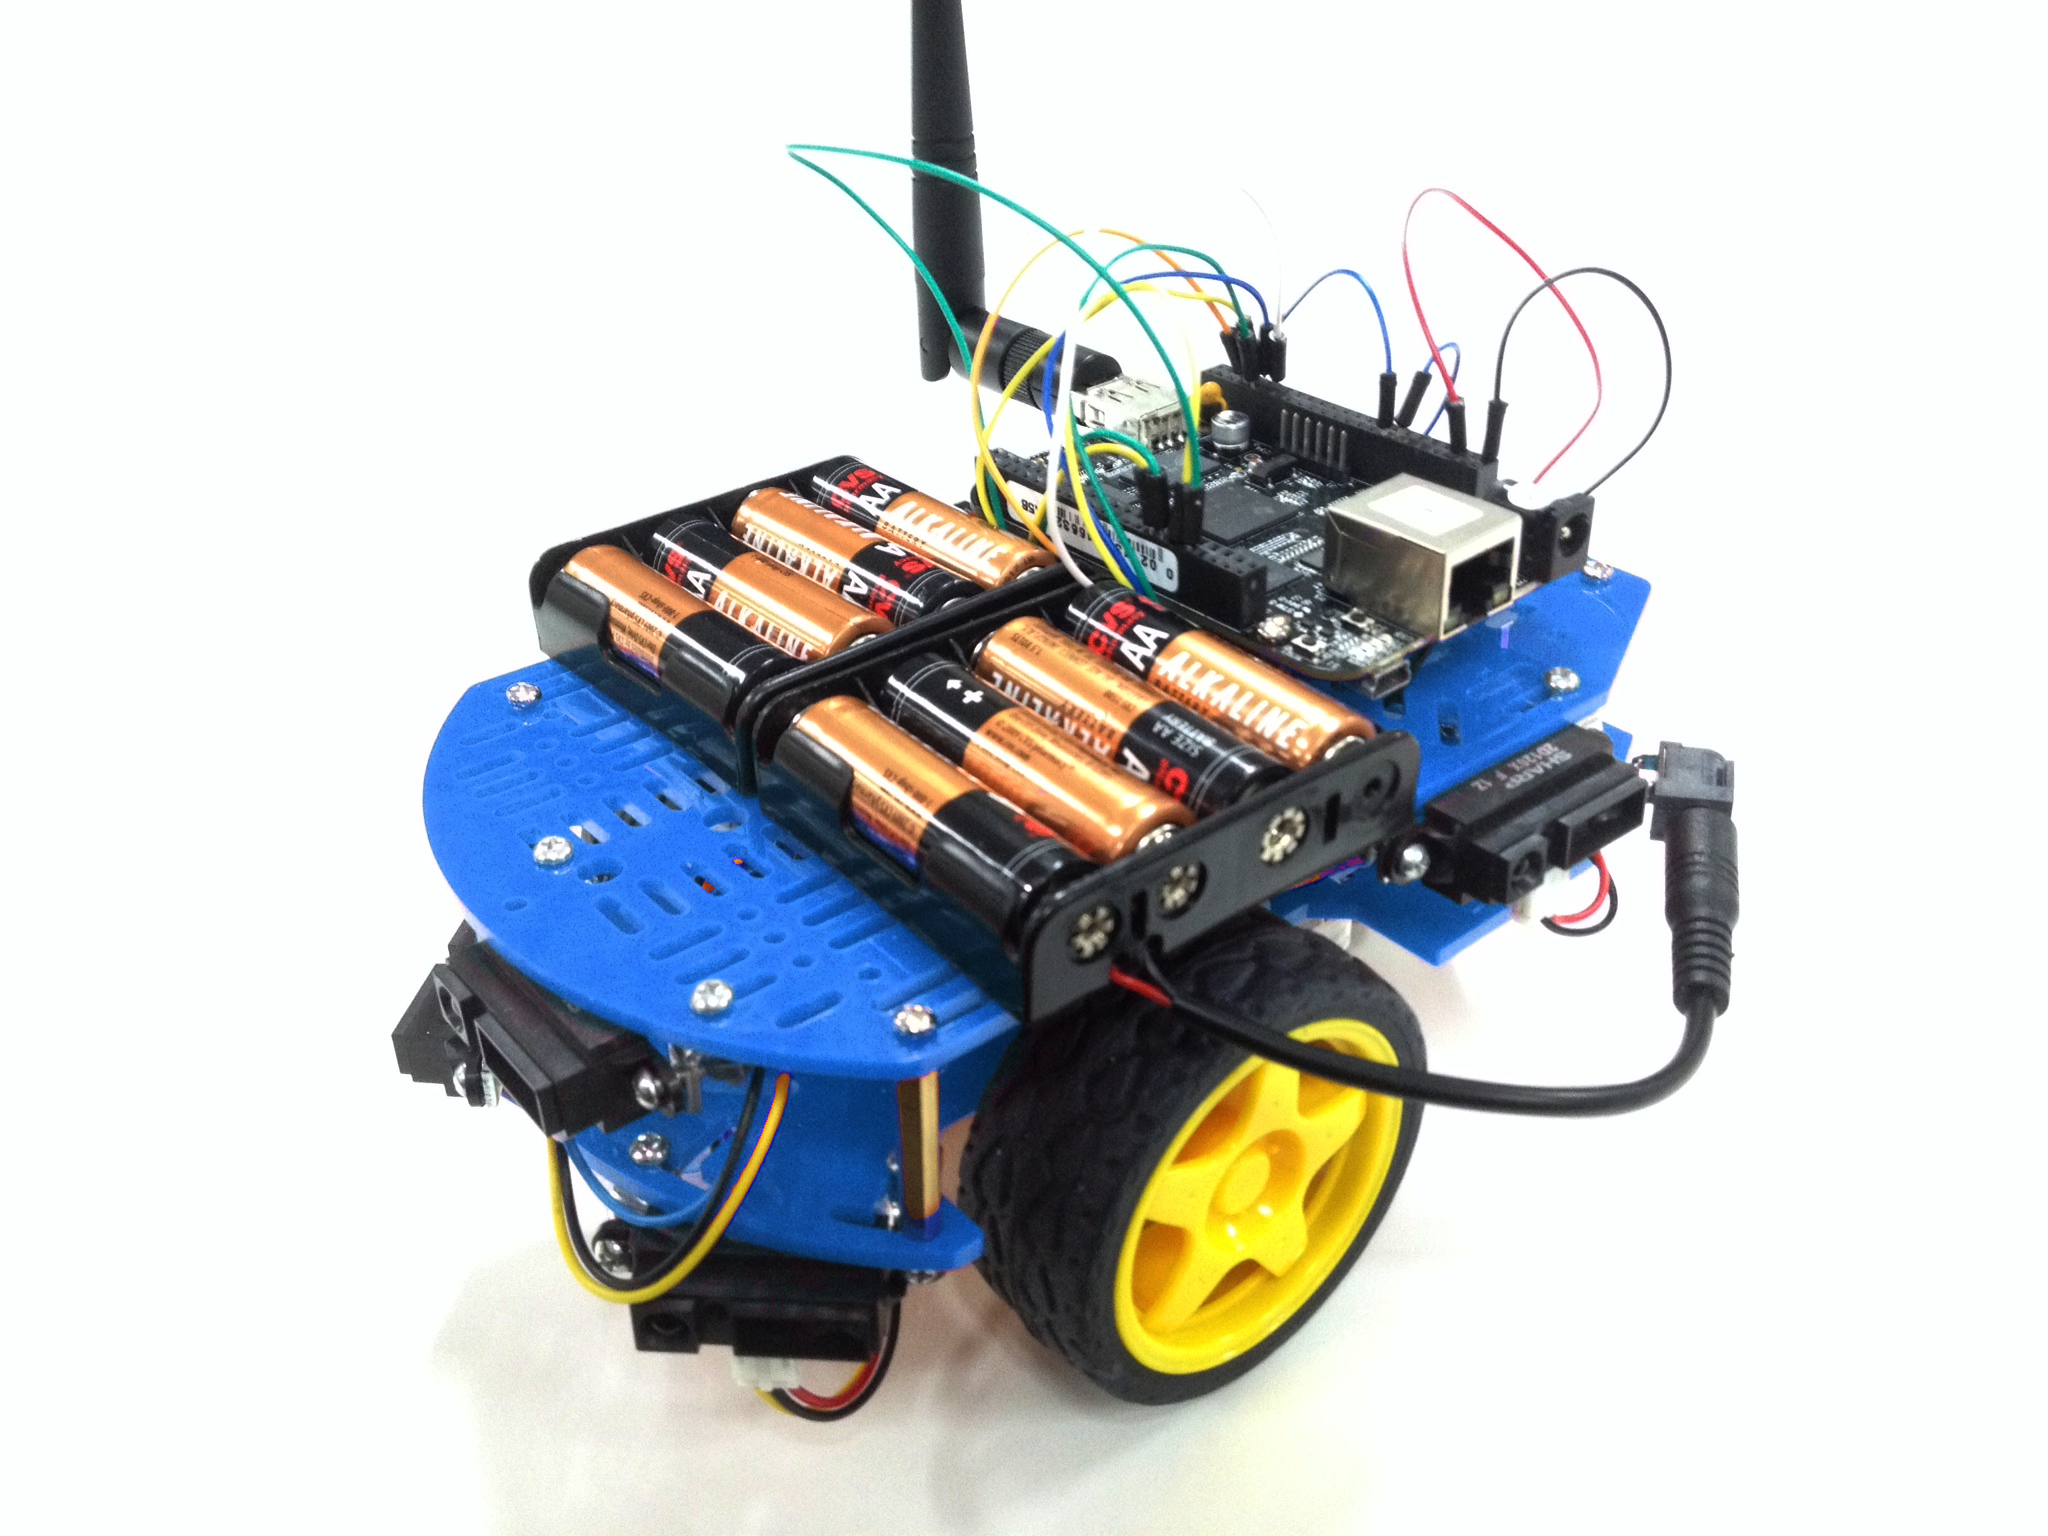
\includegraphics[trim={6cm 0cm 3cm 0cm},clip,
scale=0.09]{Figuras/quickbot-blue}
		\subcaption{Robô QuickBot}
	  	\label{fig:test2}
	\end{subfigure}
	
	\textbf{Fonte: \citeonline{im:Khepera}, \citeonline{im:QuickBot_Blue}}
\end{figure}


%		\begin{figure}[!htb]
%			\centering
%			\caption{Robôs Khepera e QuickBot fisicamente e em simulação}
%			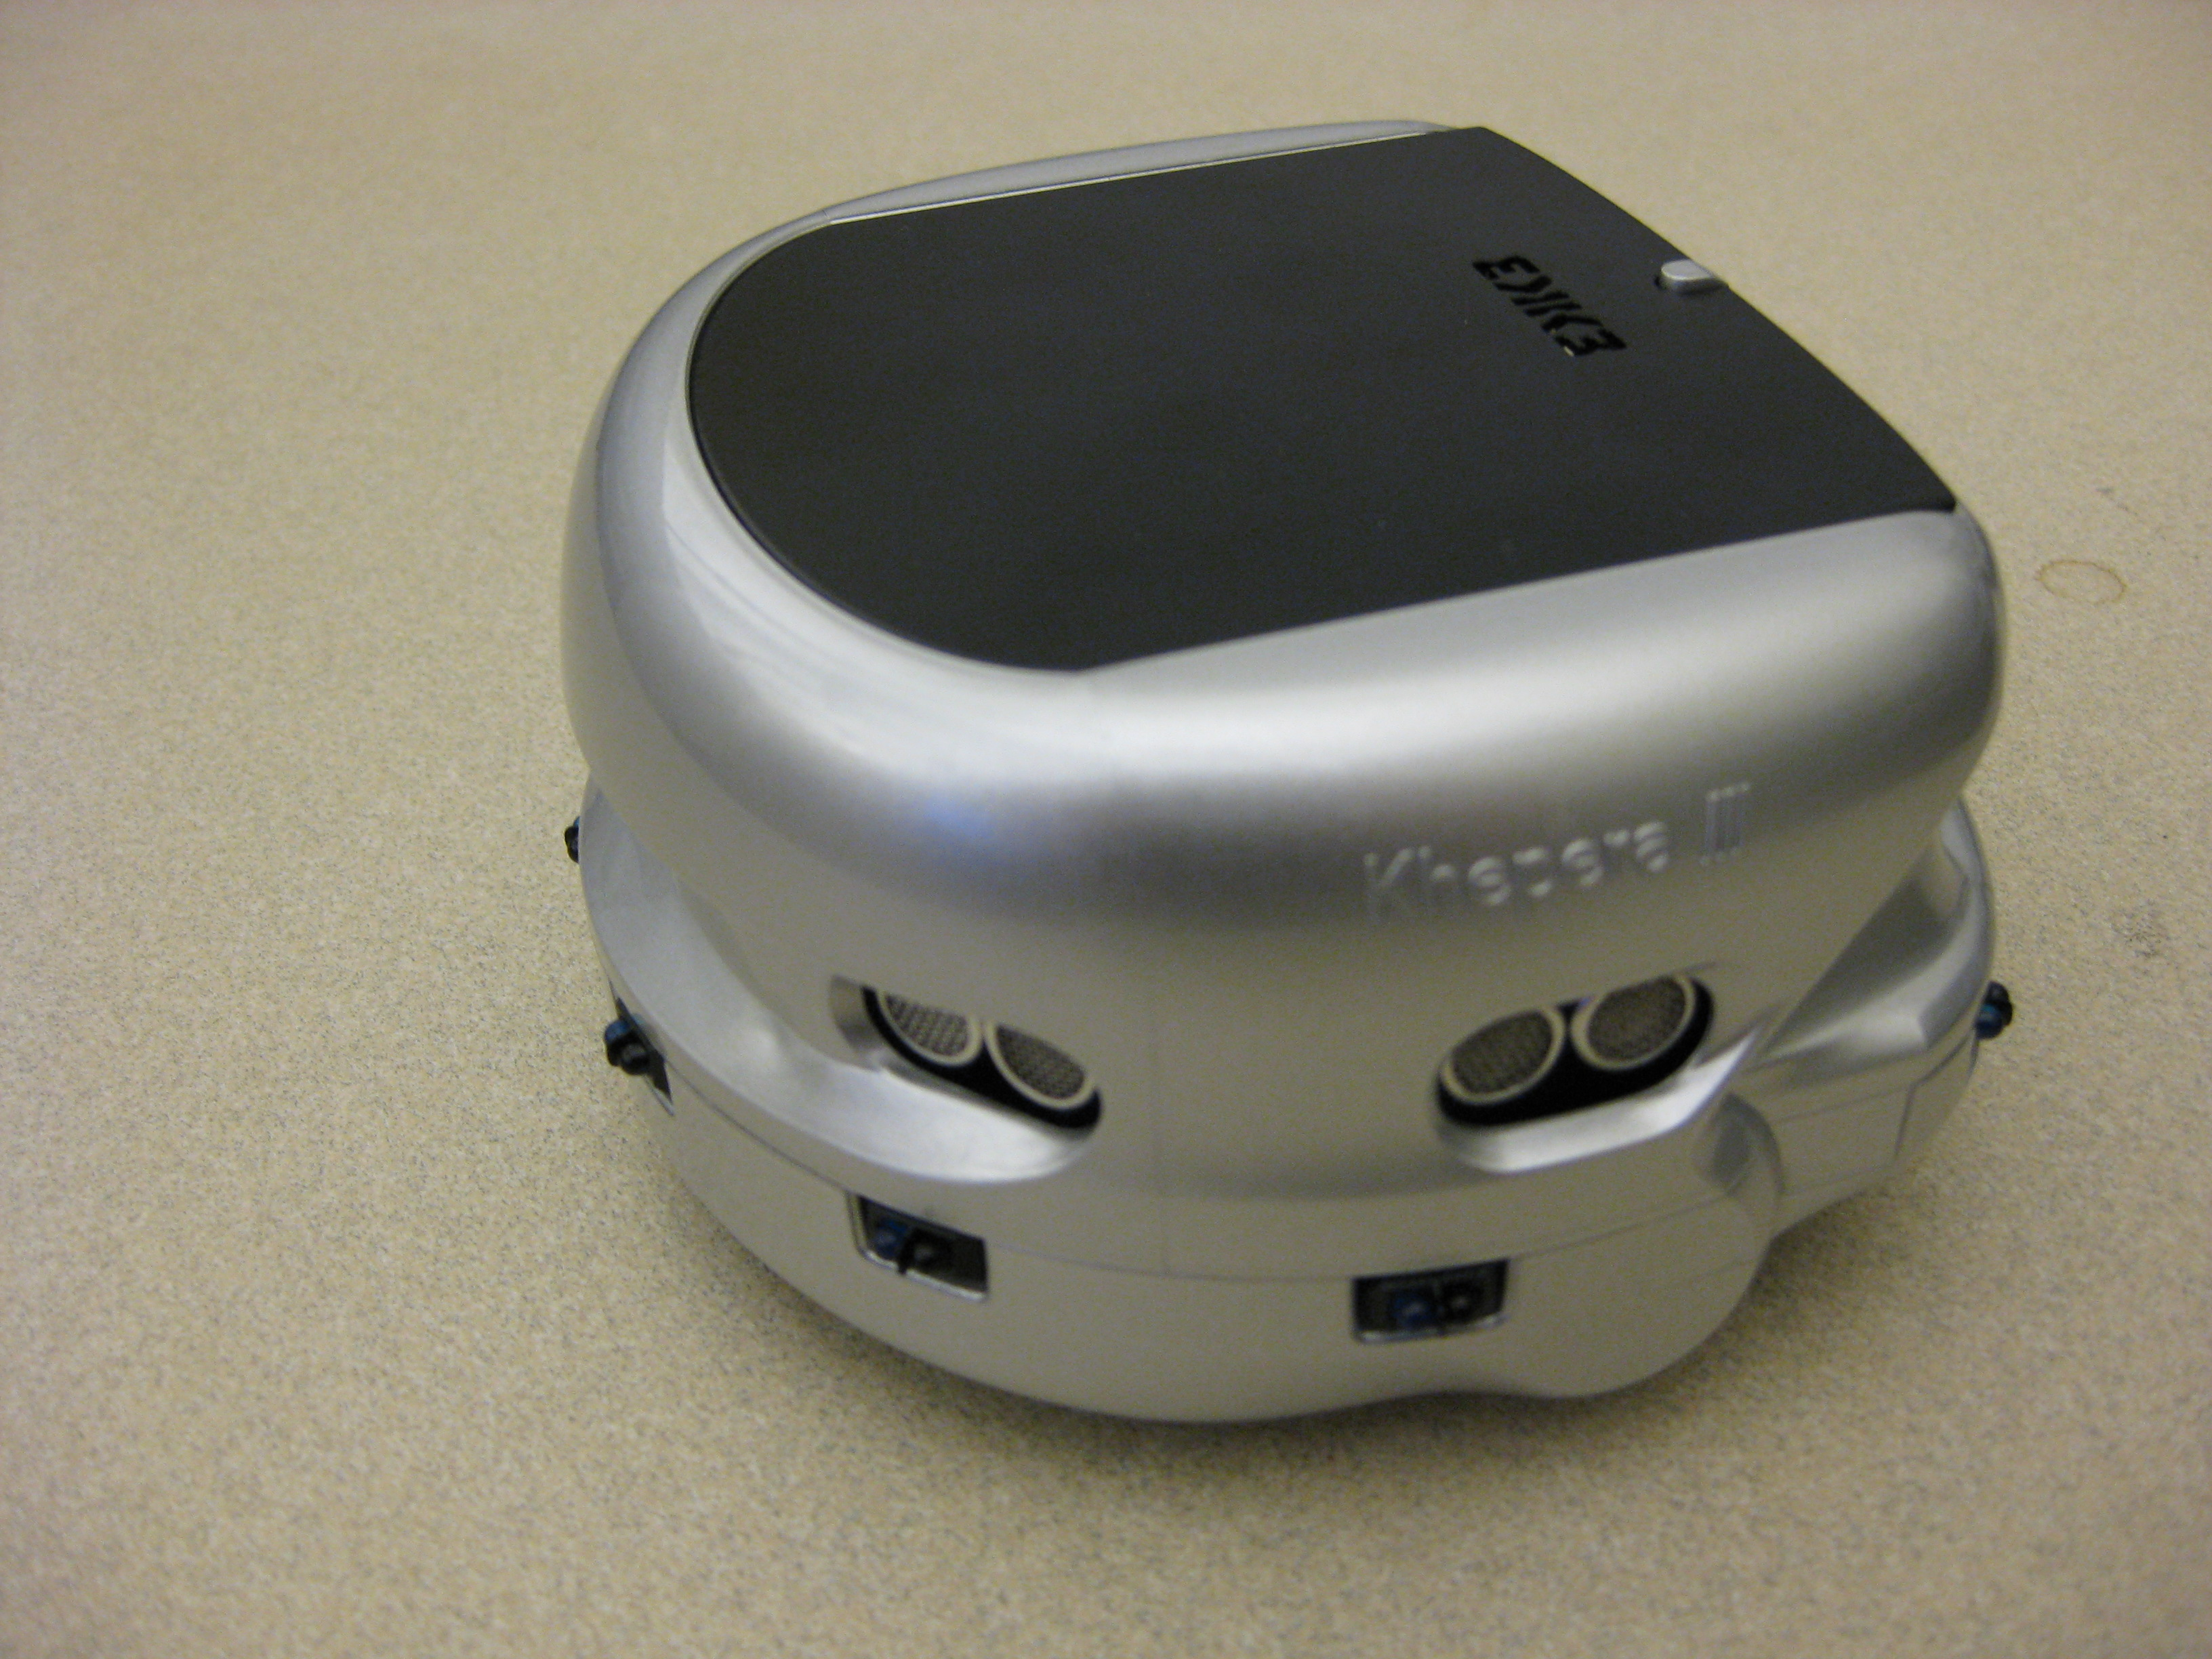
\includegraphics[trim={0cm 0cm 0cm 0cm},clip,
%scale=0.35]{Figuras/Khepera_III_robot}
%			%\vspace{-0.4cm}
%			\label{fig:RobosESim}
%		\end{figure}

%		\begin{figure}[!htb]
%			\centering			
%			\caption{Robôs Khepera e QuickBot fisicamente e em simulação}
%			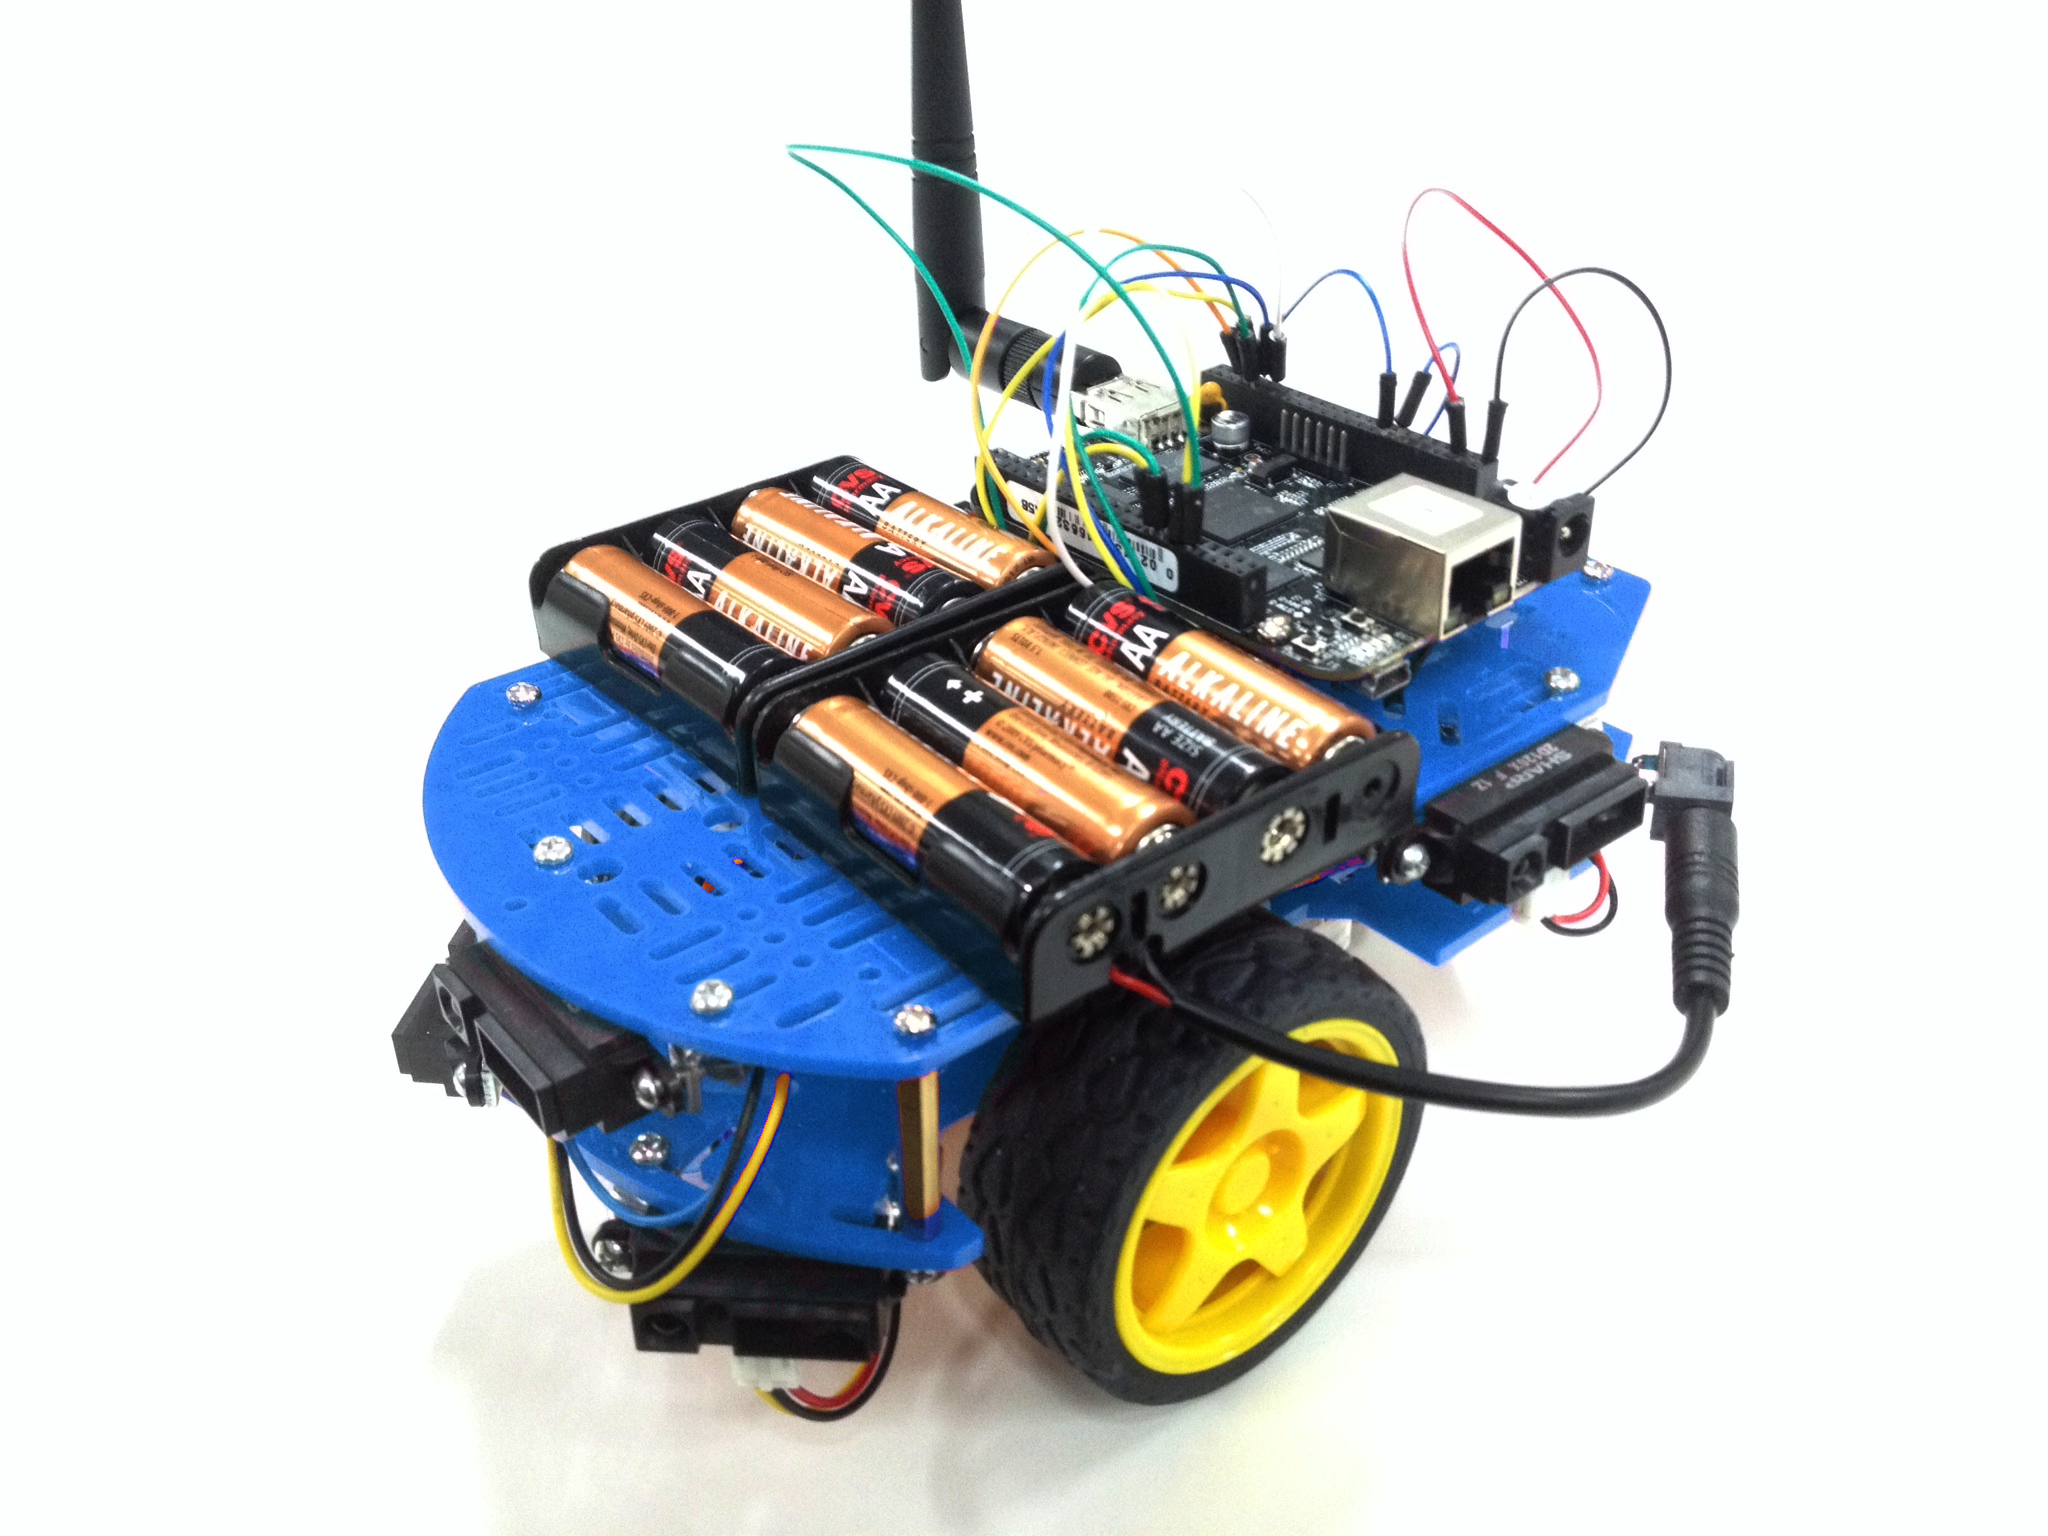
\includegraphics[trim={0cm 0cm 0cm 0cm},clip,
%scale=0.25]{Figuras/quickbot-blue}
%			%\vspace{-0.4cm}
%			\label{fig:RobosESim}
%		\end{figure}

%		\begin{figure}[!htb]
%			\centering
%			\caption{Robôs Khepera e QuickBot fisicamente e em simulação}
%			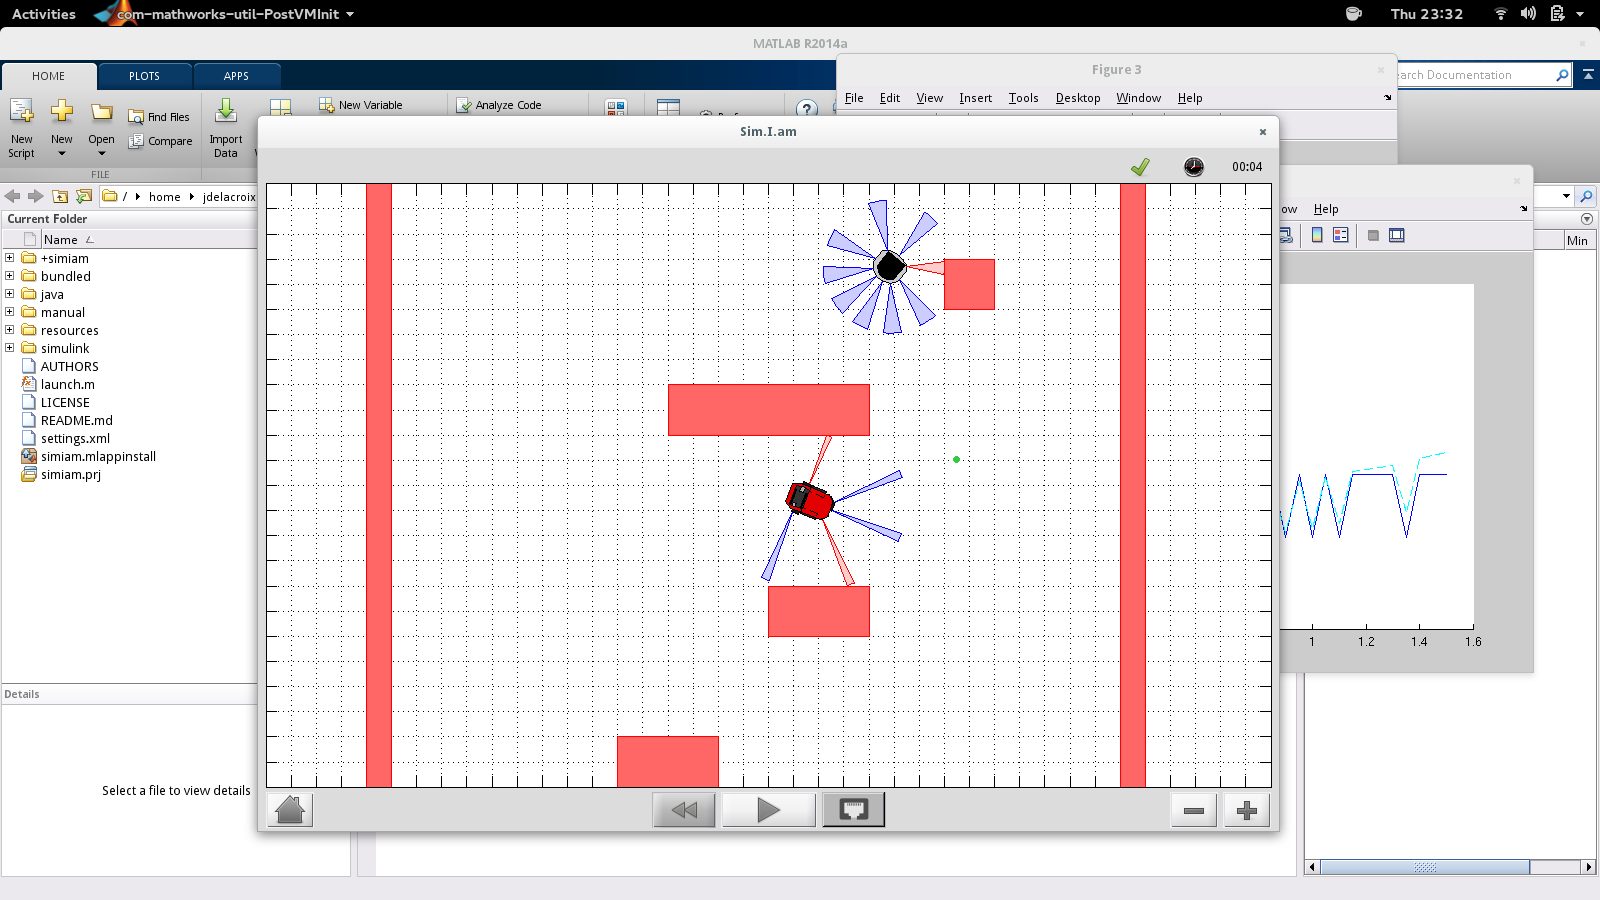
\includegraphics[trim={0cm 0cm 0cm 0cm},clip,
%scale=0.25]{Figuras/simiam-screenshot}
%			%\vspace{-0.4cm}
%			\label{fig:RobosESim}
%		\end{figure}


%\begin{figure}
%\begin{minipage}[c][11cm][t]{.5\textwidth}
%  \vspace*{\fill}
%  \centering
%  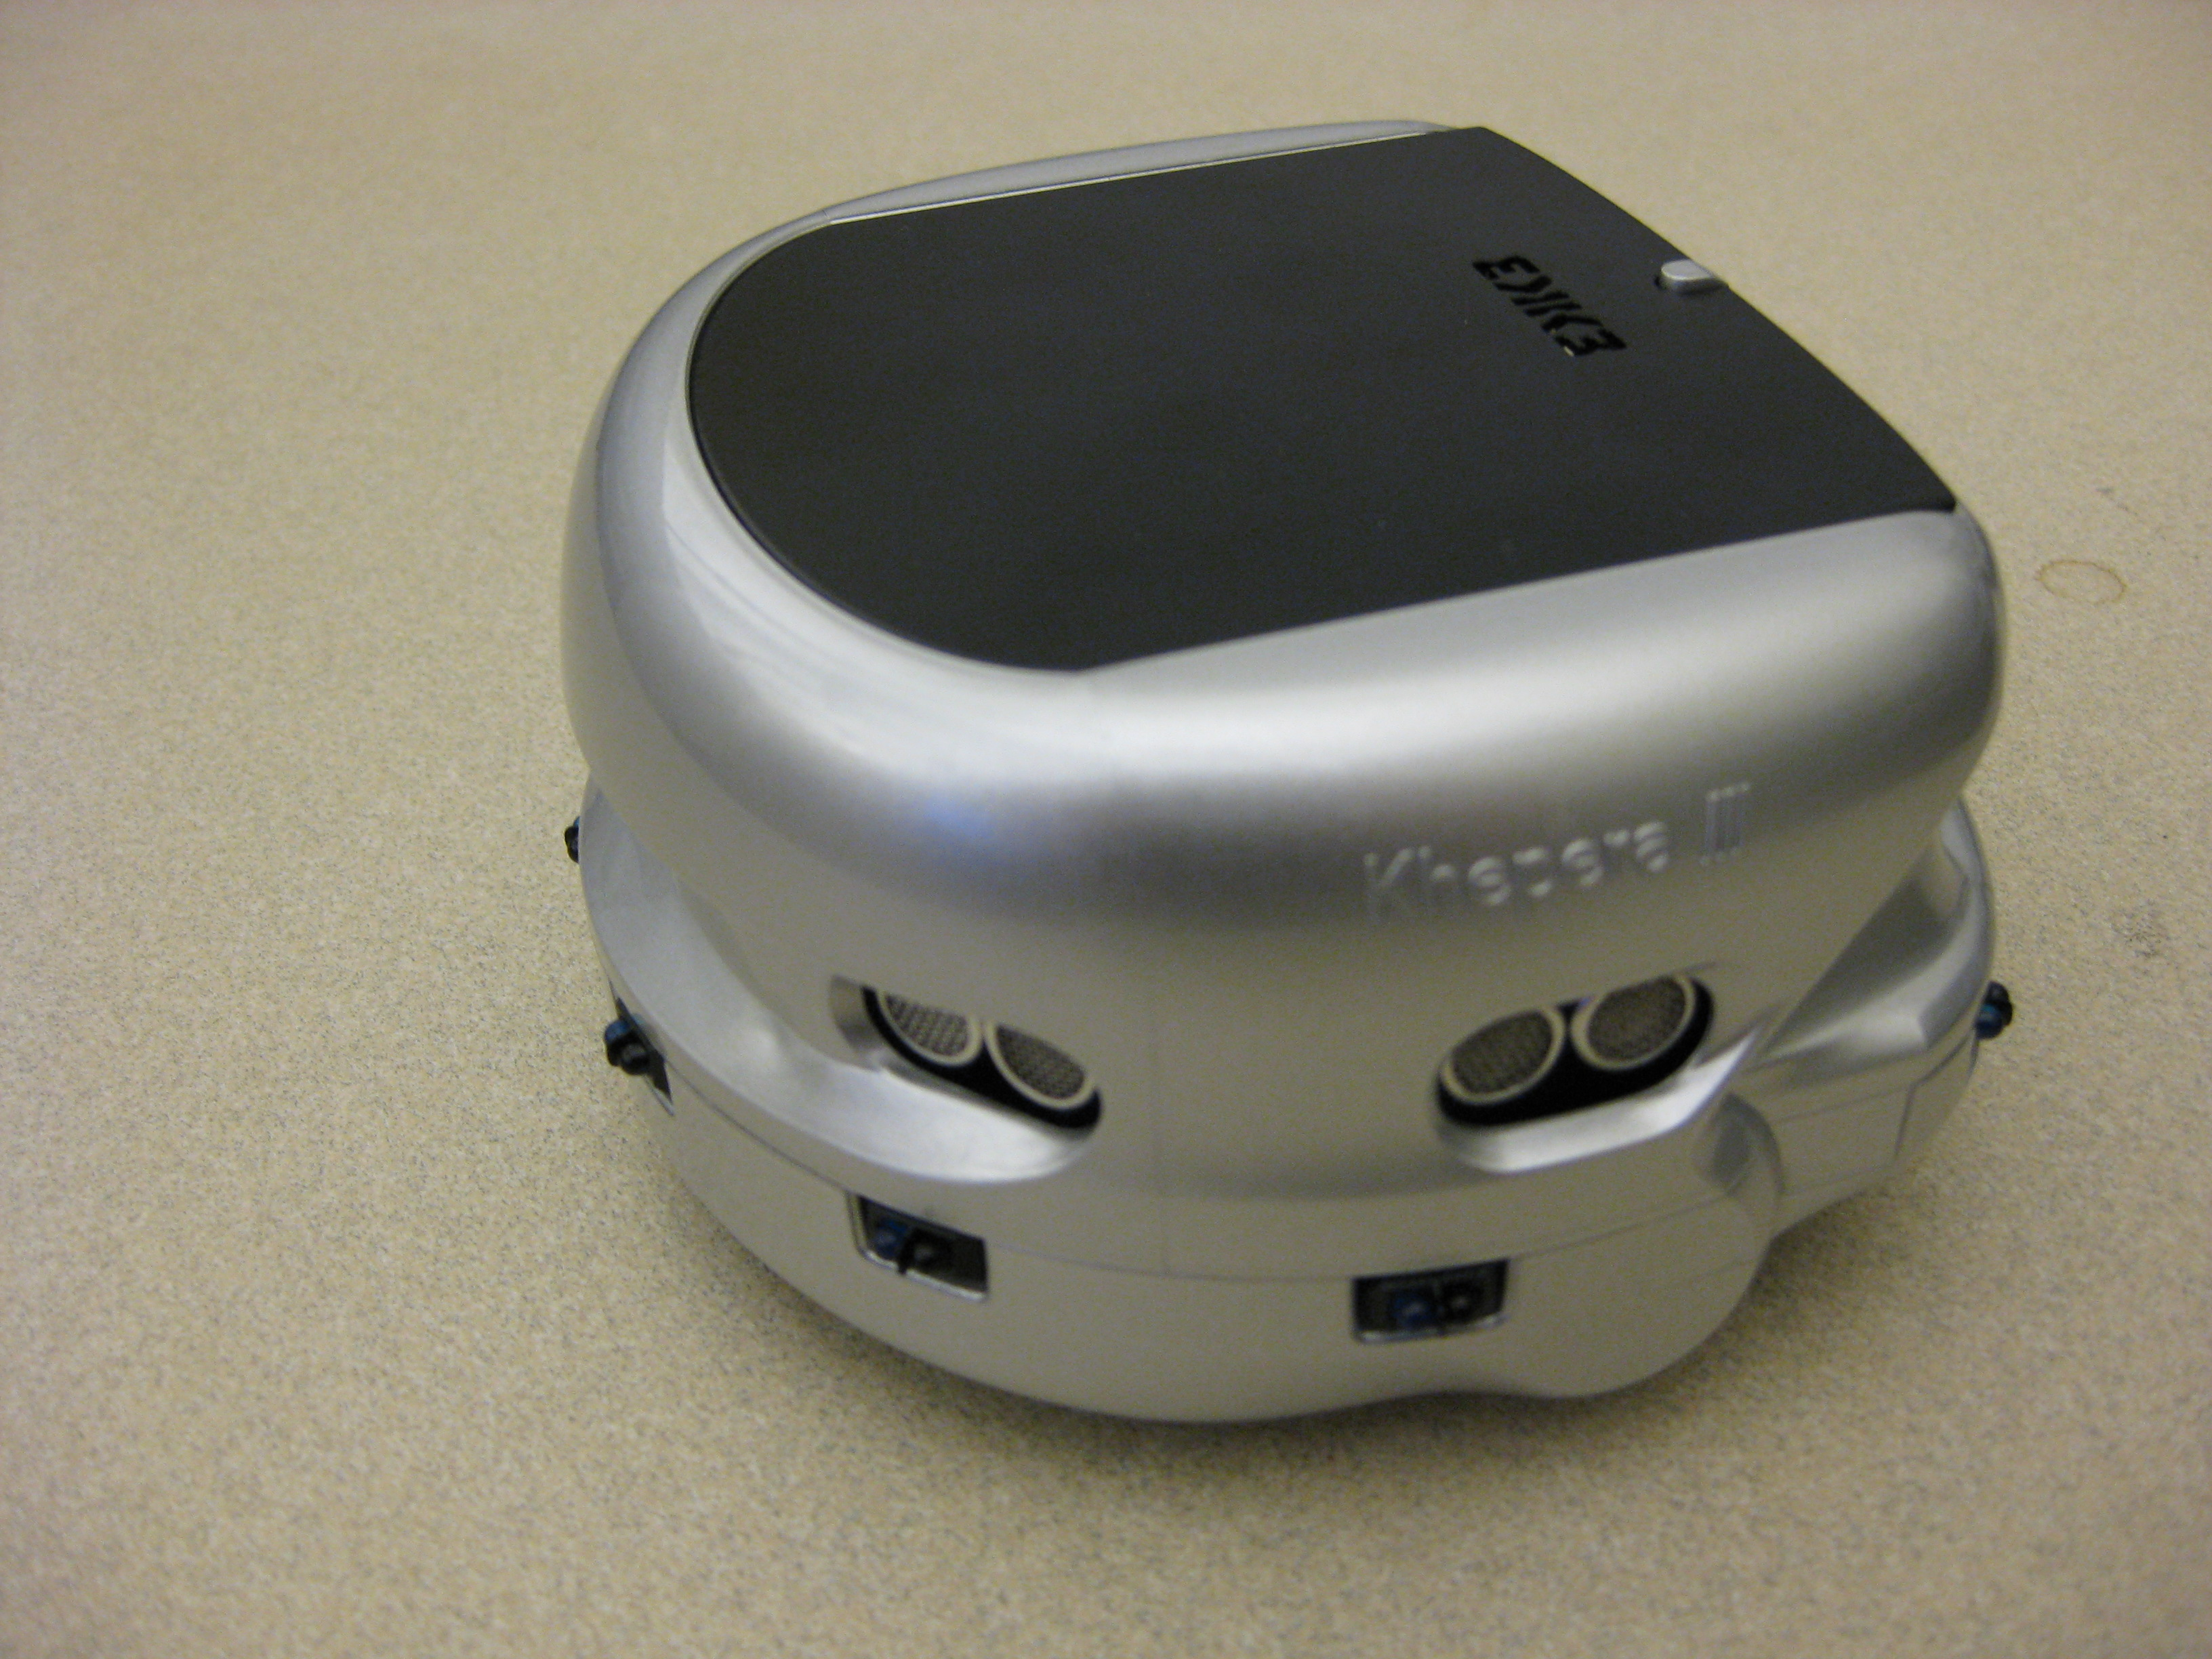
\includegraphics[width=5cm,height=4.5cm]{Figuras/Khepera_III_robot}
%  \subcaption{Robô Khepera}
%  \label{fig:test2}\par\vfill
%  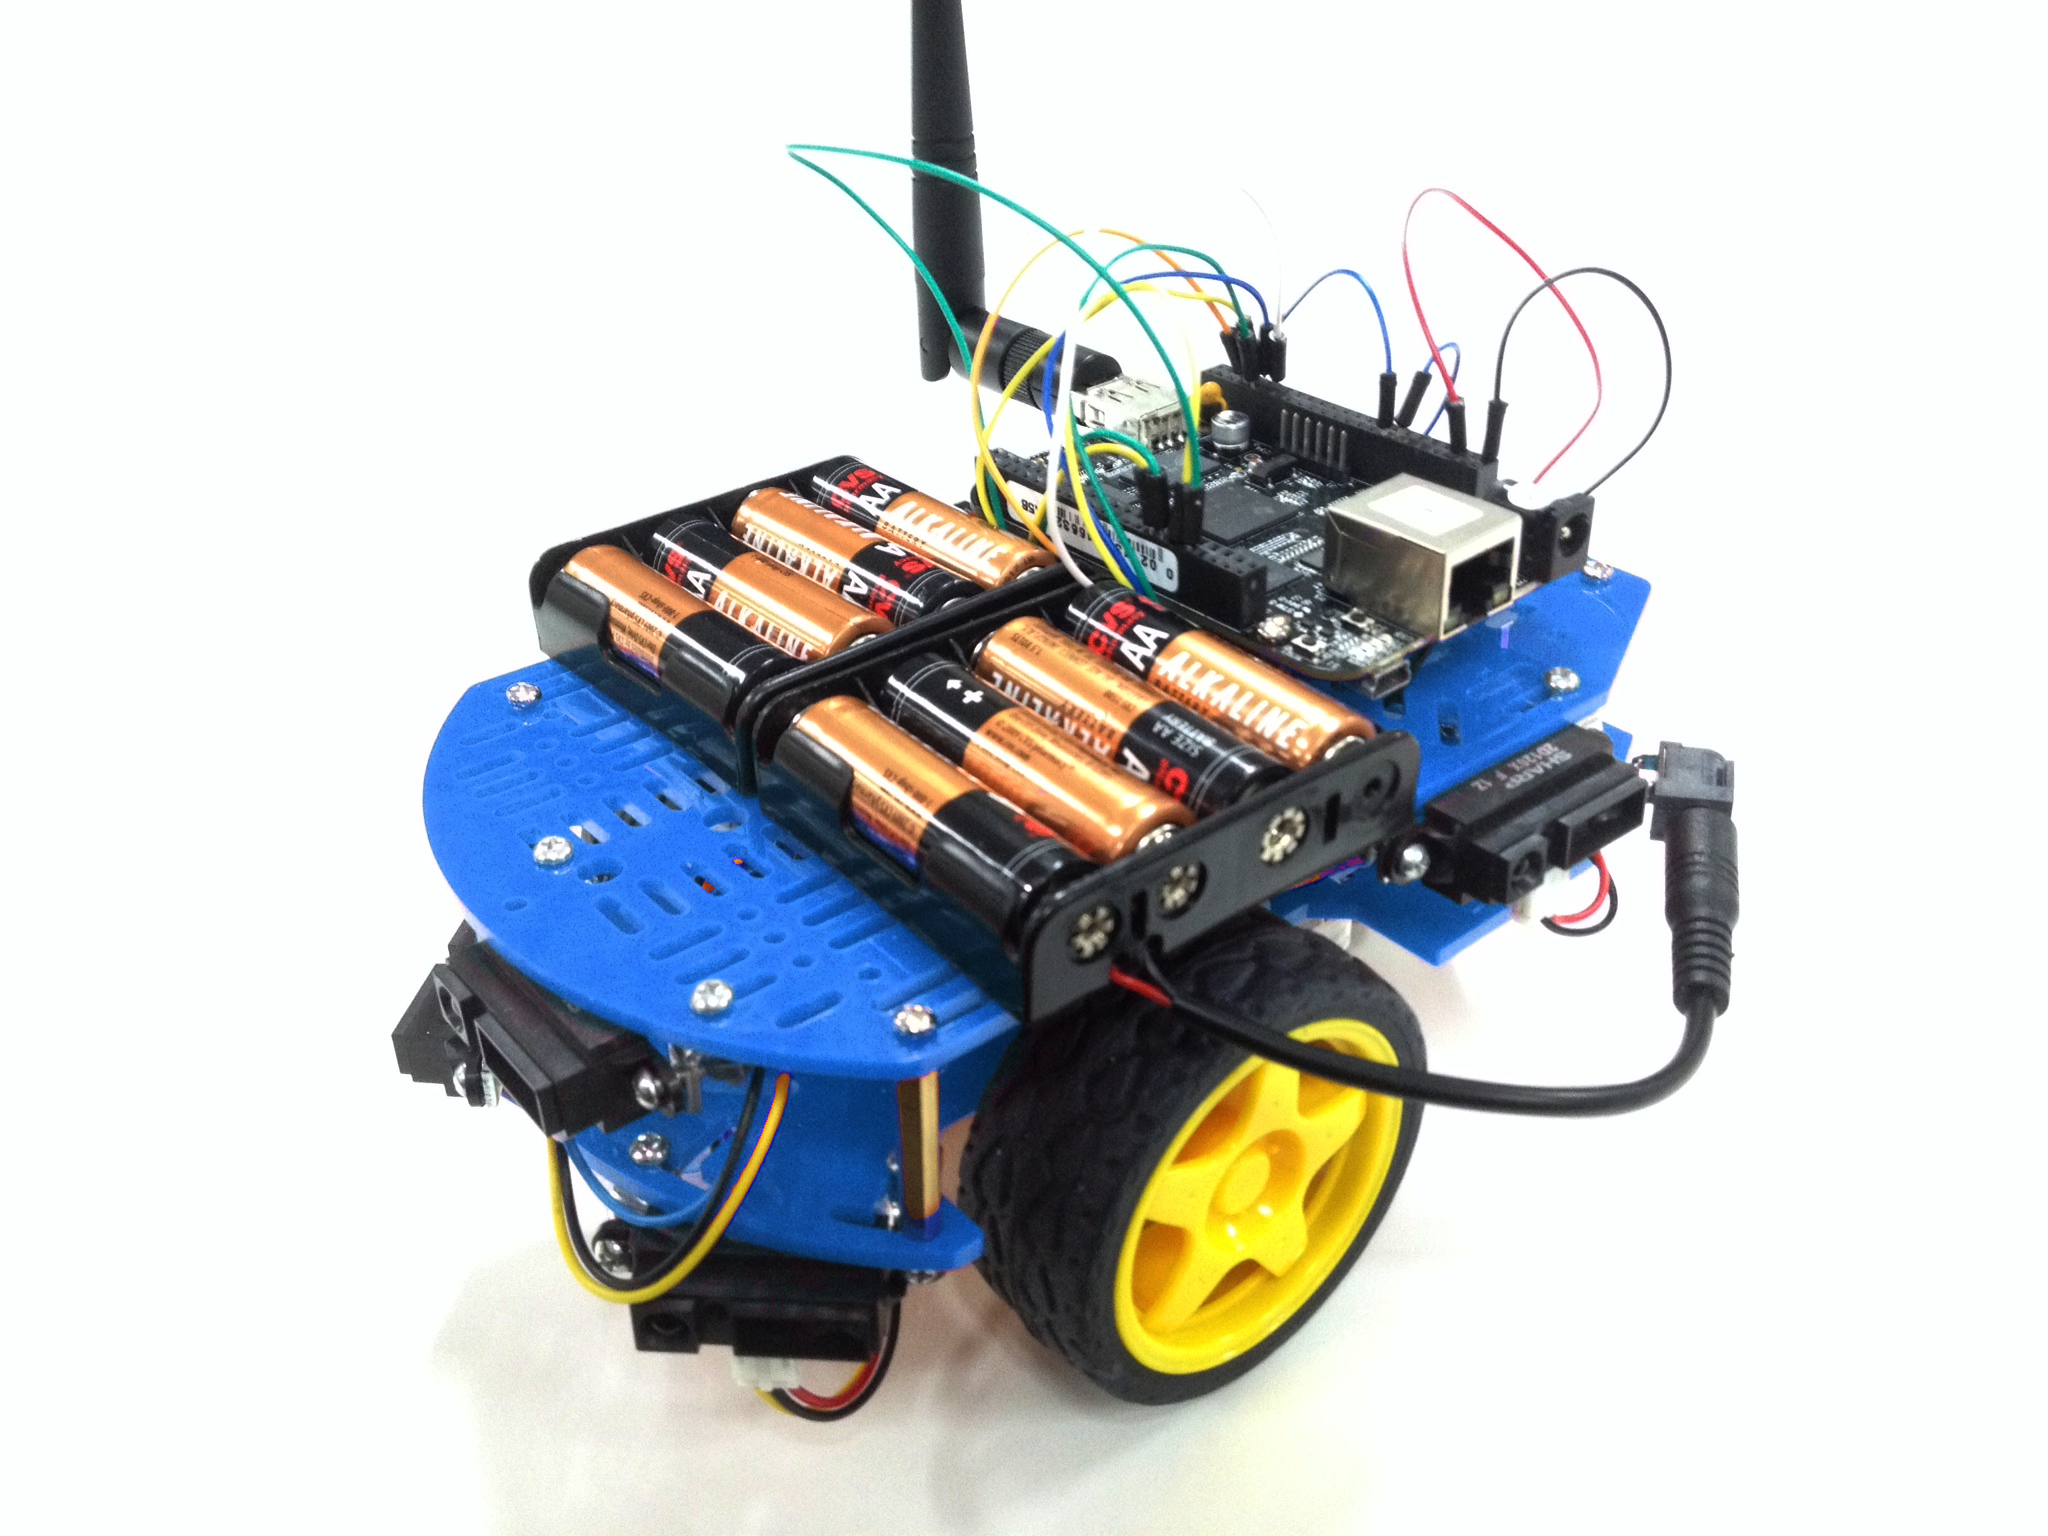
\includegraphics[width=5cm,height=4.5cm]{Figuras/quickbot-blue}
%  \subcaption{Robô QuickBot}
%  \label{fig:test3}
%\end{minipage}
%\begin{minipage}[c][11cm][t]{.5\textwidth}
%  \vspace*{\fill}
%  \centering
%  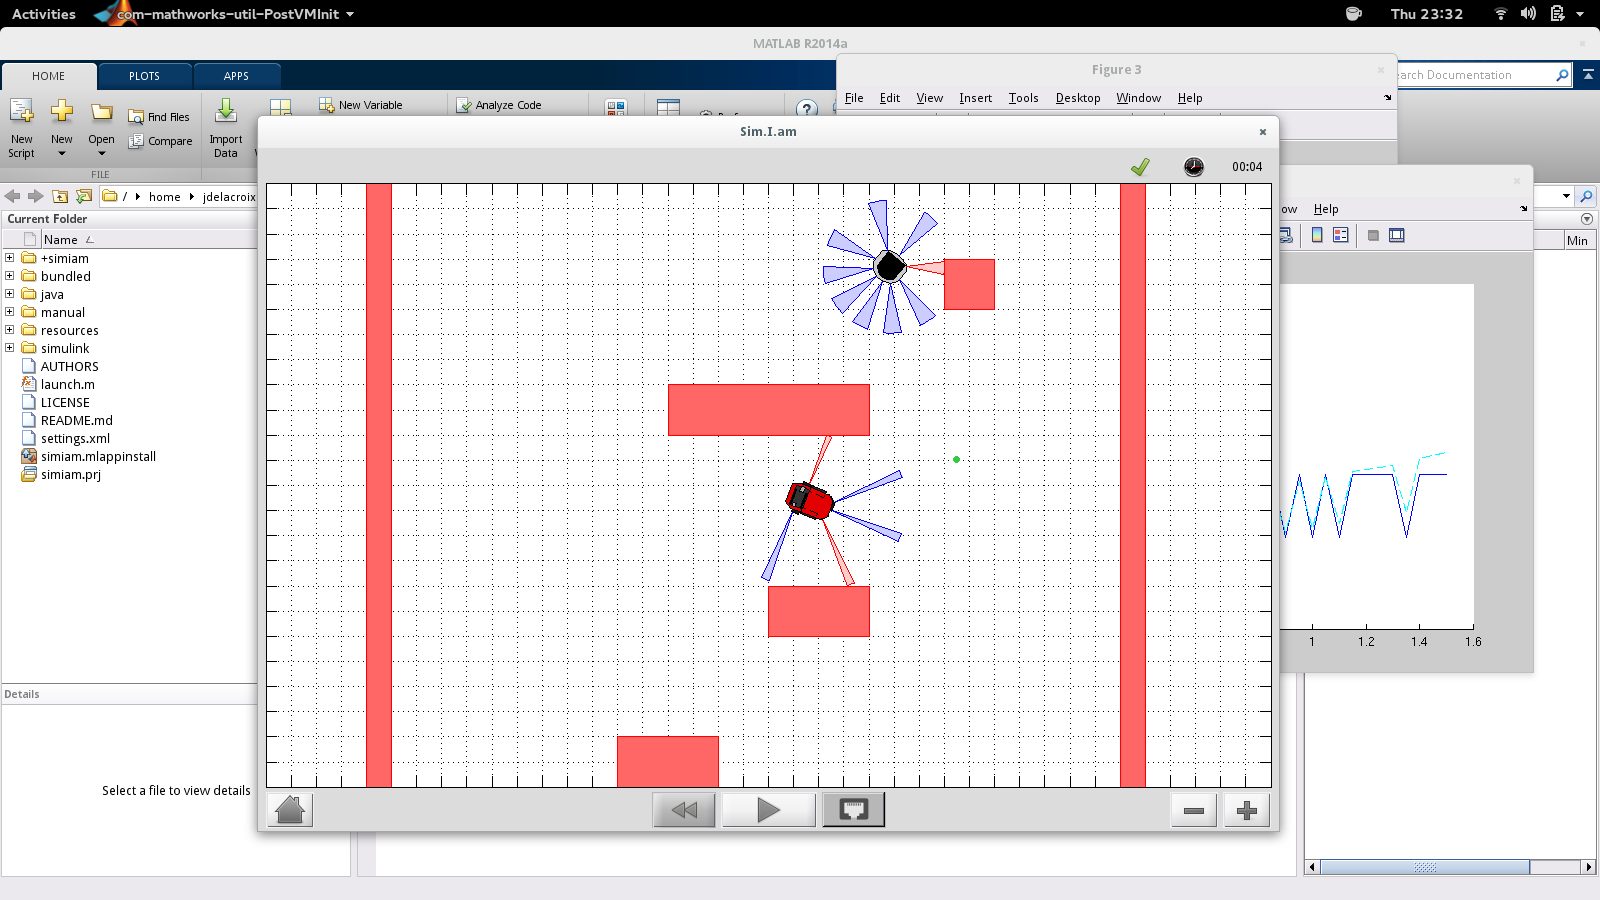
\includegraphics[width=5cm,height=10cm]{Figuras/simiam-screenshot}
%  \subcaption{Simulador Simiam}
%  \label{fig:test1}
%\end{minipage}%
%\end{figure}

\begin{figure}[ht]
\centering
\caption{Robôs Khepera 3 e QuickBot em simulação}
\label{fig:RobosEmSimulador}
		\centering
		% fbox{}
		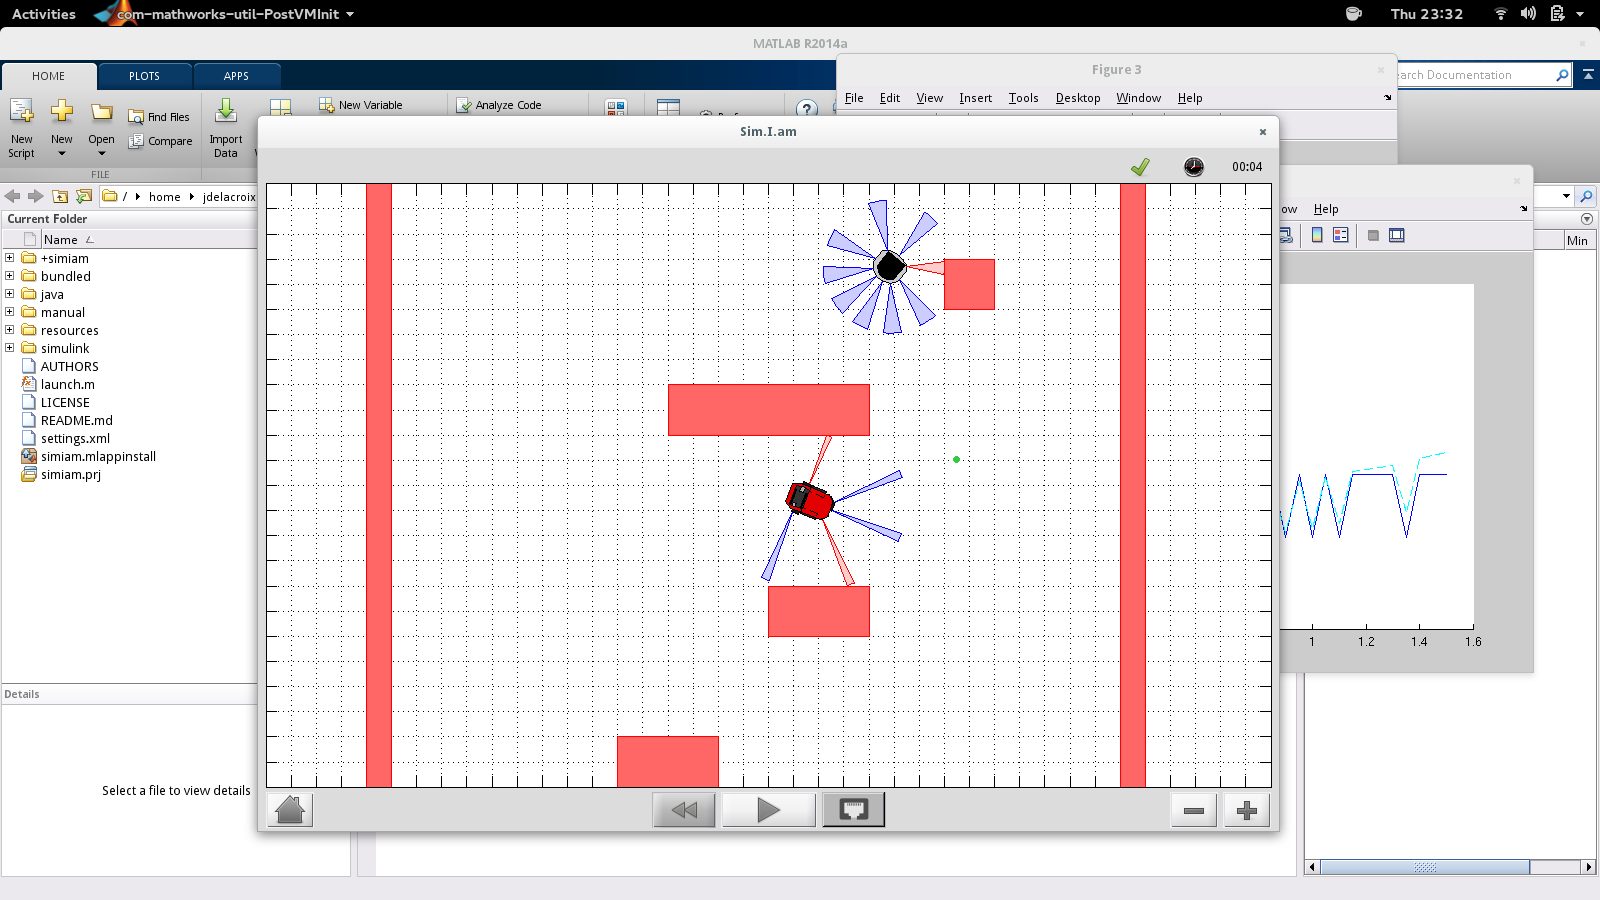
\includegraphics[trim={0cm 0cm 0cm 0cm},clip,
scale=0.24]{Figuras/simiam-screenshot}
	
	\textbf{Fonte: \citeonline{im:Simiam}}
\end{figure}

O Simiam é implementado como um aplicativo Matlab. Possui uma interface
gráfica intuitiva e uma arquitetura interna simples, facilmente customizável. As
subseções a seguir apresentam os pacotes mais importantes, bem como as
principais classes que os compõem e chama atenção para as alterações necessárias
a fim de tornar a simulação coerente com o presente trabalho.

	\subsubsection{Pacote ``ui''}
	
	O pacote ``ui'' é responsável pela interface gráfica do simulador. A classe
	``AppWindow'' possui um método construtor que inicializa atributos e o
	método ``load\_ui'' que invoca o método ``create\_layout", responsável por
	criar o leiaute da interface.
	
	O botão start, criado pelo método anterior é tratado por ``ui\_button\_start".
	Esta é a função principal reponsável por criar o ambiente de simulação
	(definido no arquivo ``settings.xml''), inserir um ou mais robôs e iniciar a
	simulação.
	
	Alterações mínimas foram efetuadas nesta etapa. Foram adicionados comandos para
	maximizar a janela do simulador e para ajustar o ``zoom'' de modo a permitir uma
	visão panorâmica de todo o ambiente de simulação. O arquivo de configuração
	``settings.xml'' foi alterado a fim de ajustar o ``tamanho do mundo'' ao
	tamanho da	tela.
	
	\subsubsection{Pacote ``simulator''}
	
	O pacote ``simulator'' realiza de fato a simulação. A classe ``World'' é
	responsável por extrair informações do arquivo ``.xml'', como quantidade e
	localização inicial de robôs e obstáculos, armazenado em estruturas de dados.
	A classe ``Simulator'' atualiza a simulação na janela, enquanto a
	classe ``Physics'' é responsável por detectar colisões de robôs com obstáculos
	e entre si. 
	
	As alterações neste pacote foram todas na classe ``Simulator'', no intuito
	de possibilitar a captura da simulação em video ``.mp4" ou ``.gif". Apesar de
	não ser uma alteração fundamental para a etapa de execução do trabalho, é
	necessária para a apresentação. Não foi criado um botão na interface para
	especificar ao simulador a captura em video. Assim, é necessário, no
	construtor da classe Simulator, atribuir valor verdadeiro aos atributos
	``gravarvideo'' e/ou ``gravargif". 
	
	\subsubsection{Pacote ``robot''}
	
	O pacote ``robot'' define um ou mais robôs passíveis de serem instanciados. A
	classe ``QuickBot'' estabelece parâmetros físicos, tais como informações
	geométricas, posicionamento dos sensores no corpo do robô e estabelece
	limitações, como velocidades de saturação e zona morta dos motores. Além de
	instanciar objetos das classes ``DifferentialDrive'', ``ProximitySensor'' e
	``WheelEncoder'', ``QuickBot'' extende a classe ``Robot''. 
	
	A classe ``DifferentialDrive" implementa a ``dinâmica'' dos modelos de
	acionamento diferencial e uniciclo. Com os métodos ``uni\_to\_diff'' e ``diff\_to\_uni'', a
	equivalência com o modelo apresentado na Equação \ref{eq:vw_to_diff} é
	estabelecida no espaço de simulação. 

	A classe ``ProximitySensor'' estabelece características do sensor infravermelho
	usado no QuickBot, tais como distâncias mínimas e máximas, espalhamento, localização e
	direção em relação ao corpo do robô e adiciona um ruído gaussiano.
	``WheelEncoder'', similarmente, estabelece características do \textit{encoder}.
	
	As alterações nesta etapa foram no intuito de incluir o robô deste trabalho
	no Simiam. O arquivo ``settings.xml'' deve determinar que um objeto (robô) da
	nova classe criada seja instanciado, ao invés do objeto da classe QuickBot.
	
	\subsubsection{Pacote ``controller''}
	
	O pacote ``controller'' é responsável pela implementação de todos os
	controladores e supervisores dos robôs implementados. A classe ``Supervisor'' é
	extendida para obter o controlador supervisório de cada robô a ser simulado.
	Para o QuickBot e Khepera 3, os respectivos supervisores são definidos pelas
	classes ``QBSupervisor'' e ``K3Supervisor''. Essas classes definem máquinas de
	estado, onde cada estado é associado a um controlador de variável contínua.
	Esses controladores, por sua vez, extendem a classe ``Controller'' e
	implementam os ``comportamentos'', ou modos, dos robôs.
	% Calculo de odometria está em QBSupervisor.
	
	As alterações neste pacote foram responsáveis pela inclusão de suporte a
	controladores \textit{Fuzzy}, além de adicionar o supervisório específico para
	o robô desenvolvido.

\subsection{Especificações}

As variáveis L e R na Equação \ref{eq:diff}, para o robô deste trabalho, valem
respectivamente 18 cm e 3,4 cm.

O robô deste trabalho foi feito com base no robô ``QuickBot''. Contudo, o sensor infravermelho do ``QuickBot''
é o ``GP2Y0A41SK0F'', cuja região de medição está no intervalo entre 4 e 30 cm. Por conta deste sensor estar 
obsoleto, ele foi substituído pelo ``GP2Y0A21YK0F'' que possui a curva de tensão por distância representada na 
Figura \ref{fig:SensorIR}. A faixa de distância do sensor deste trabalho está entre 10 e 80 cm, como pode ser visto
na Figura. 

\begin{figure}[ht]
	\centering
	\caption{Resposta do sensor infravermelho}
	\label{fig:SensorIR}
	
	%\fbox{}
	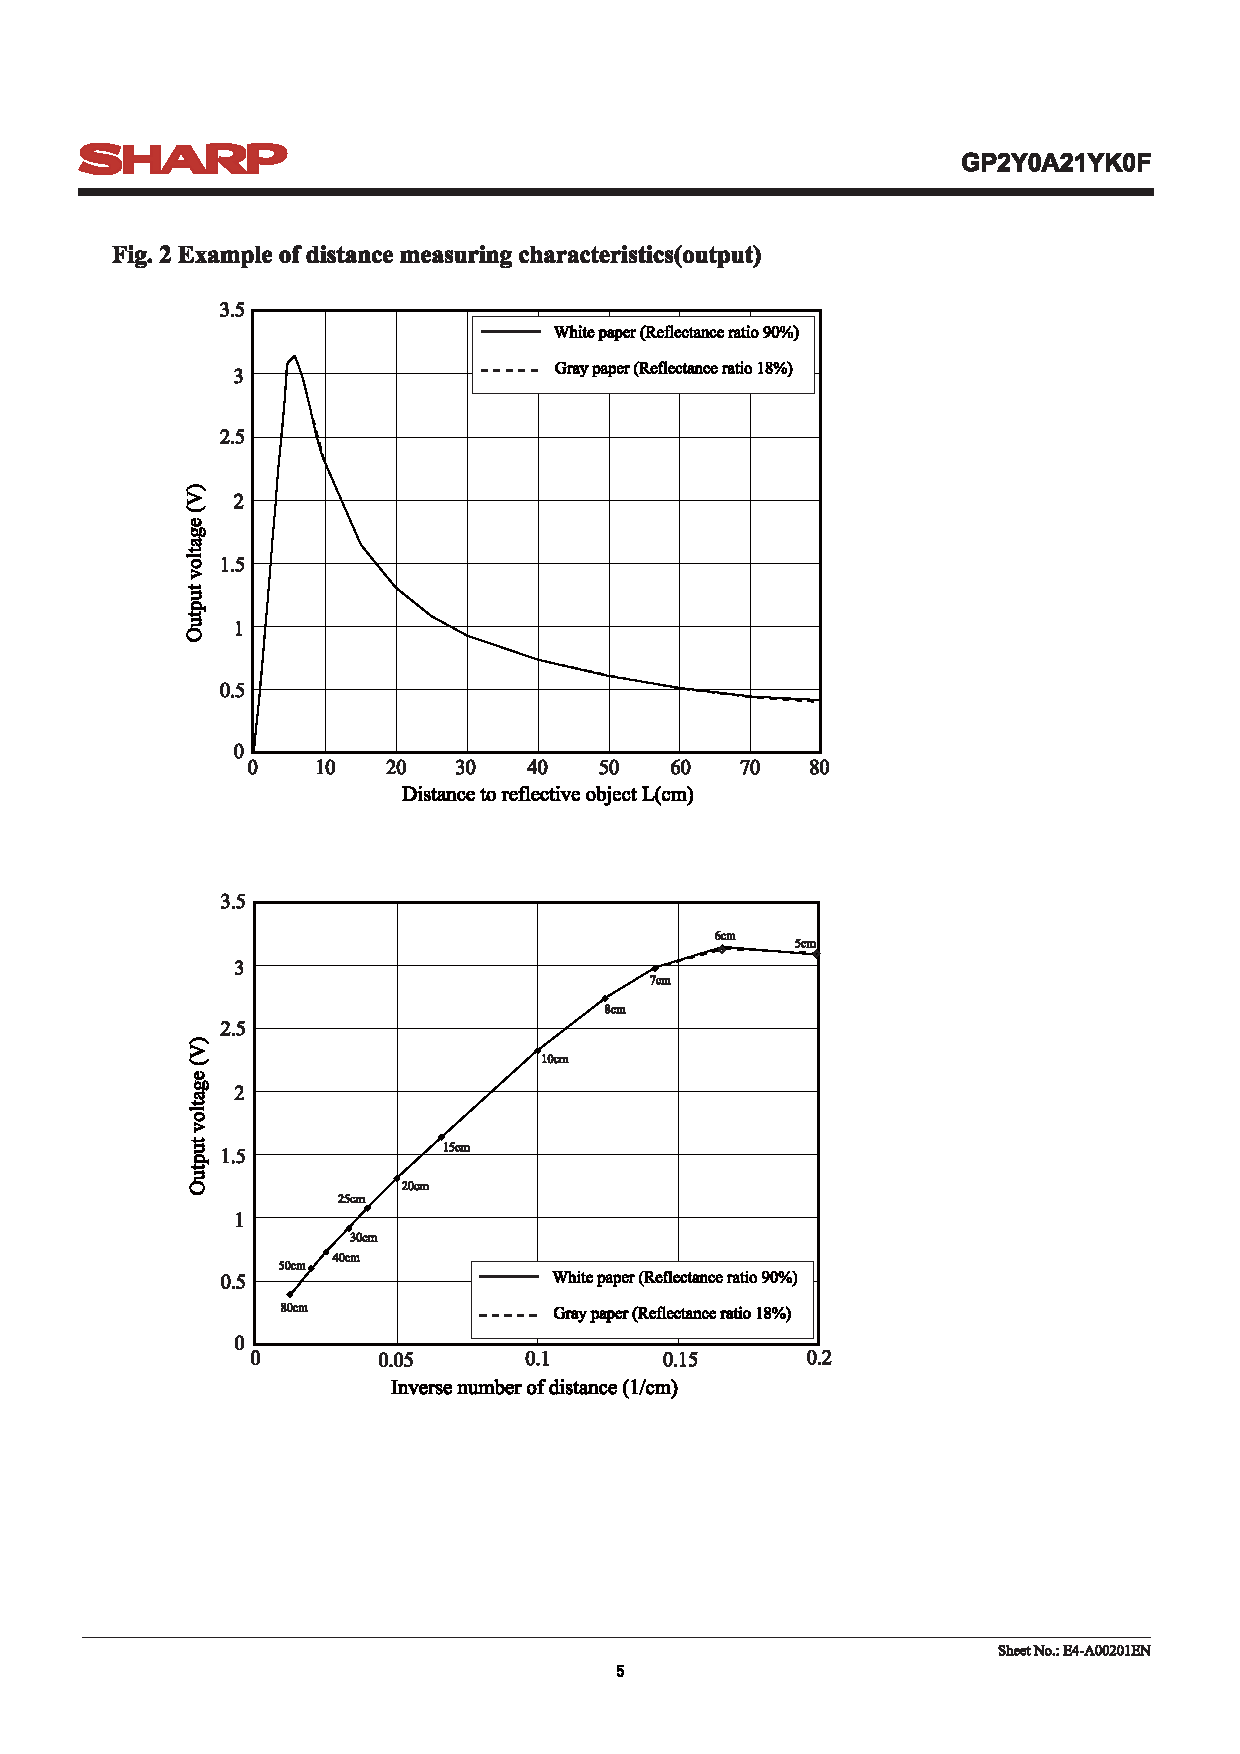
\includegraphics[trim= 3cm 15.8cm 6.5cm 4.8cm,clip,
scale=1]{Figuras/IR_Datasheet_Figure}

	%\begin{tikzpicture}[auto, node distance=2cm, on grid,
%>=latex']%
	
	%\node[anchor=south west,inner sep=0] (image) at (0,0) {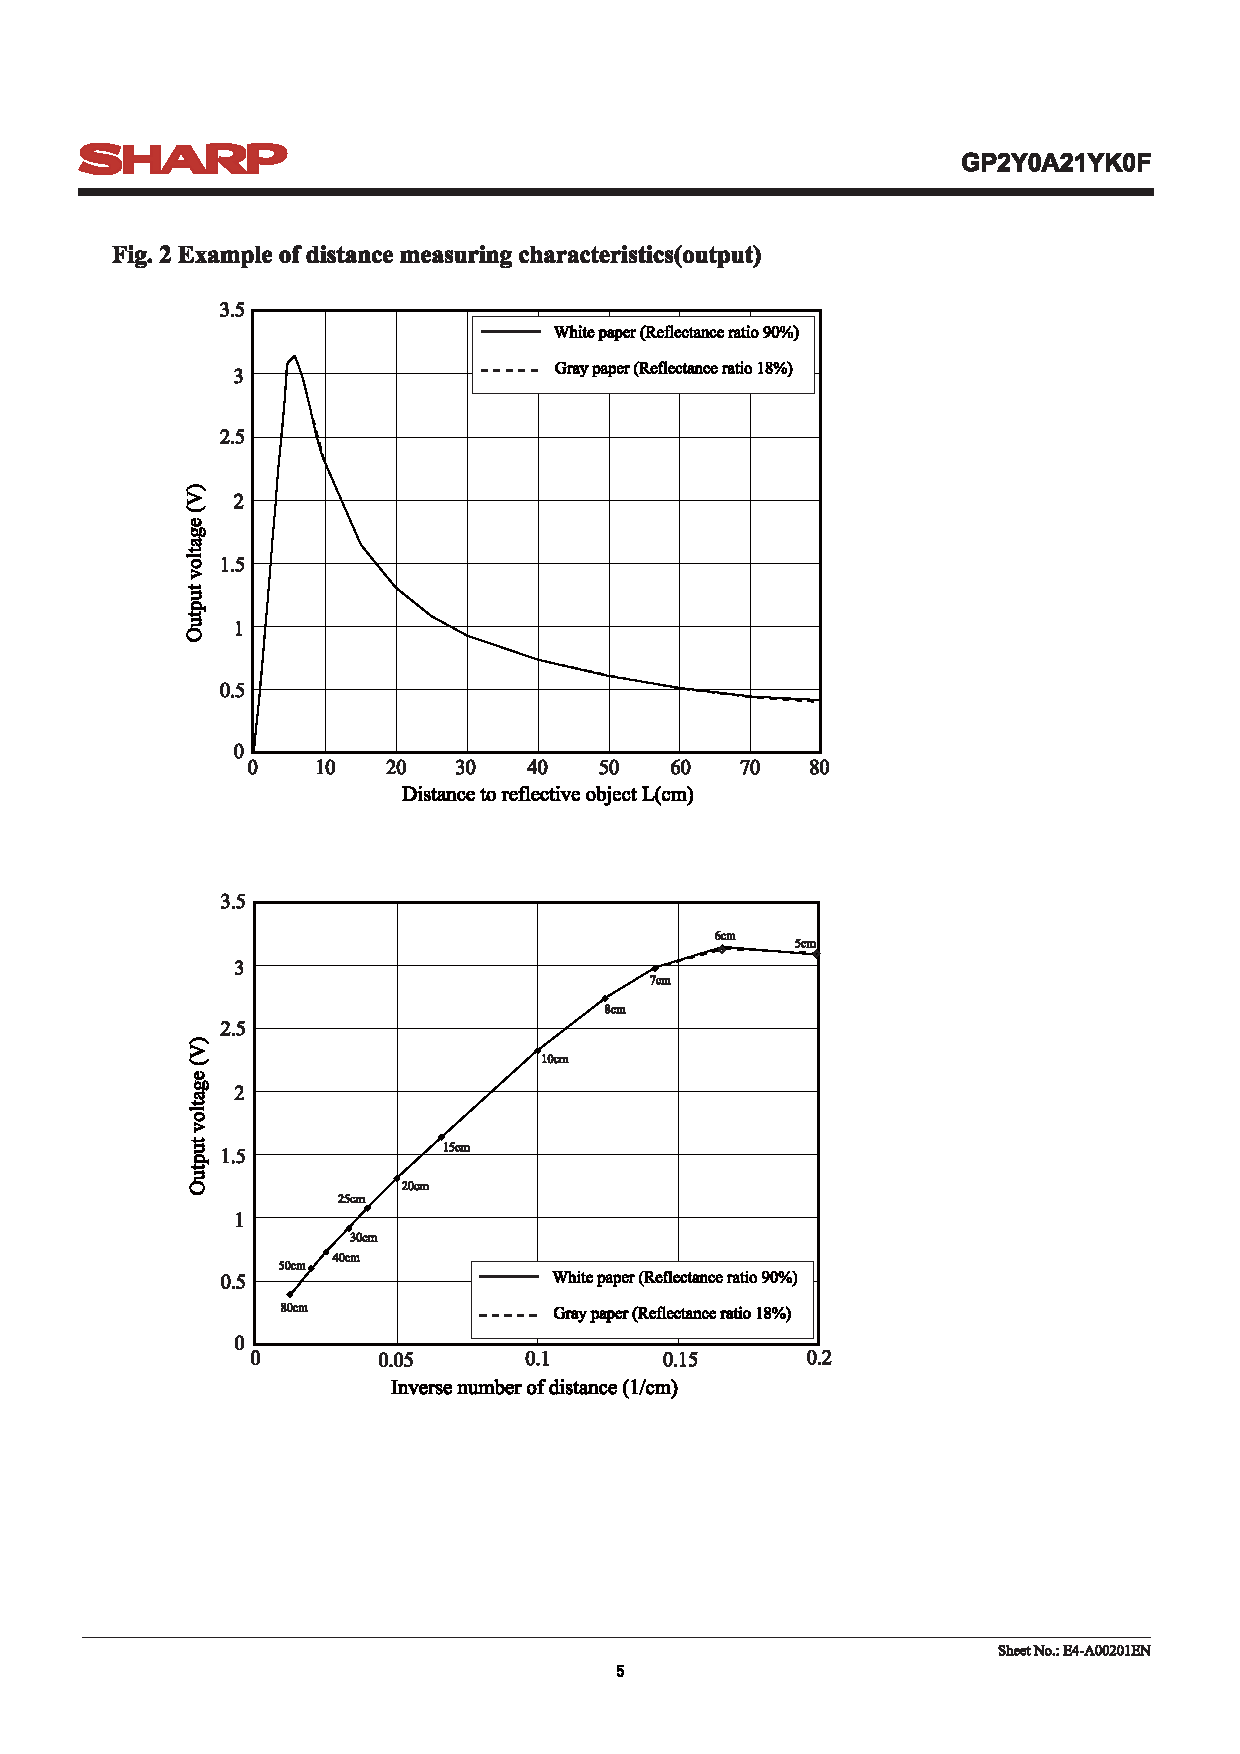
\includegraphics[trim =
%		{3cm 15.8cm 6.5cm 4.8cm}, clip,scale=1]{Figuras/IR_Datasheet_Figure}};
		
%	\node[fill,circle,inner sep=0.1pt, color = red] at (1.29,1.161) {};
%	\node[fill,circle,inner sep=0.1pt, color = red] at (2.525,2.235) {};
	
%	\node[fill,circle,inner sep=0.1pt, color = red] at (1.83,7.75) {};
	
	
%	\node[inner sep = 0 pt, outer sep = 0 pt] (origin) at (1.3,1.15) {};
%	\node[inner sep = 0 pt, outer sep = 0 pt] (teste2) at (2.55,2.25) {};
%	
%	\node[inner sep = 0 pt, outer sep = 0 pt] (P1) at (1.85,7.85) {};
	
	%\draw[-, color = red] (origin) -- (teste2);
	%\draw[-, color = red] (origin) -- (P1);
	
	%\node[] at (0,0) {};
	%\coordinate[] (teste1) {};
	%\coordinate[] (teste2) {};
	
	%\draw[-, color = red] (-18,2) -- (-7,3);
	
%	\end{tikzpicture}


	\textbf{Fonte: \citeonline{datasheet:SensorIR}}
\end{figure}

Para a região da curva onde $d > 4.95 cm$, o polinômio que a aproxima, associando
a distância pela tensão ($d(v)$), obtido utilizando a função ``polyfit'' do Matlab pode ser visto 
na Equação \ref{eq:PolinomioVx}.
\begin{equation}
	\label{eq:PolinomioVx}
	\begin{split}
		d(v) = 2.7802212625 v^6 -35.1150300110 v^5 + 179.6031433005 v^4 \\
		-477.9449116299 v^3 + 706.3400747125 v^2 -569.7367375002 v + 221.2678651473
	\end{split}
\end{equation}

\subsection{Montagem Física}

	Nesta seção pretende-se mostrar as questões práticas necessárias para a construção do 
	robô.
	
\subsubsection{Processo de montagem}

	Os componentes físicos do robô podem ser vistos na Figura \ref{fig:RoboReal}. Alguns
	números foram acrescentados às imagens ao lado dos periféricos utilizados, a fim de 
	rotulá-los.
	
	\begin{figure}[!ht]
\centering
\caption{Materiais e robô após montagem}
\label{fig:RoboReal}
	\begin{subfigure}[b]{0.49\textwidth}%
		\centering
		% fbox{}
		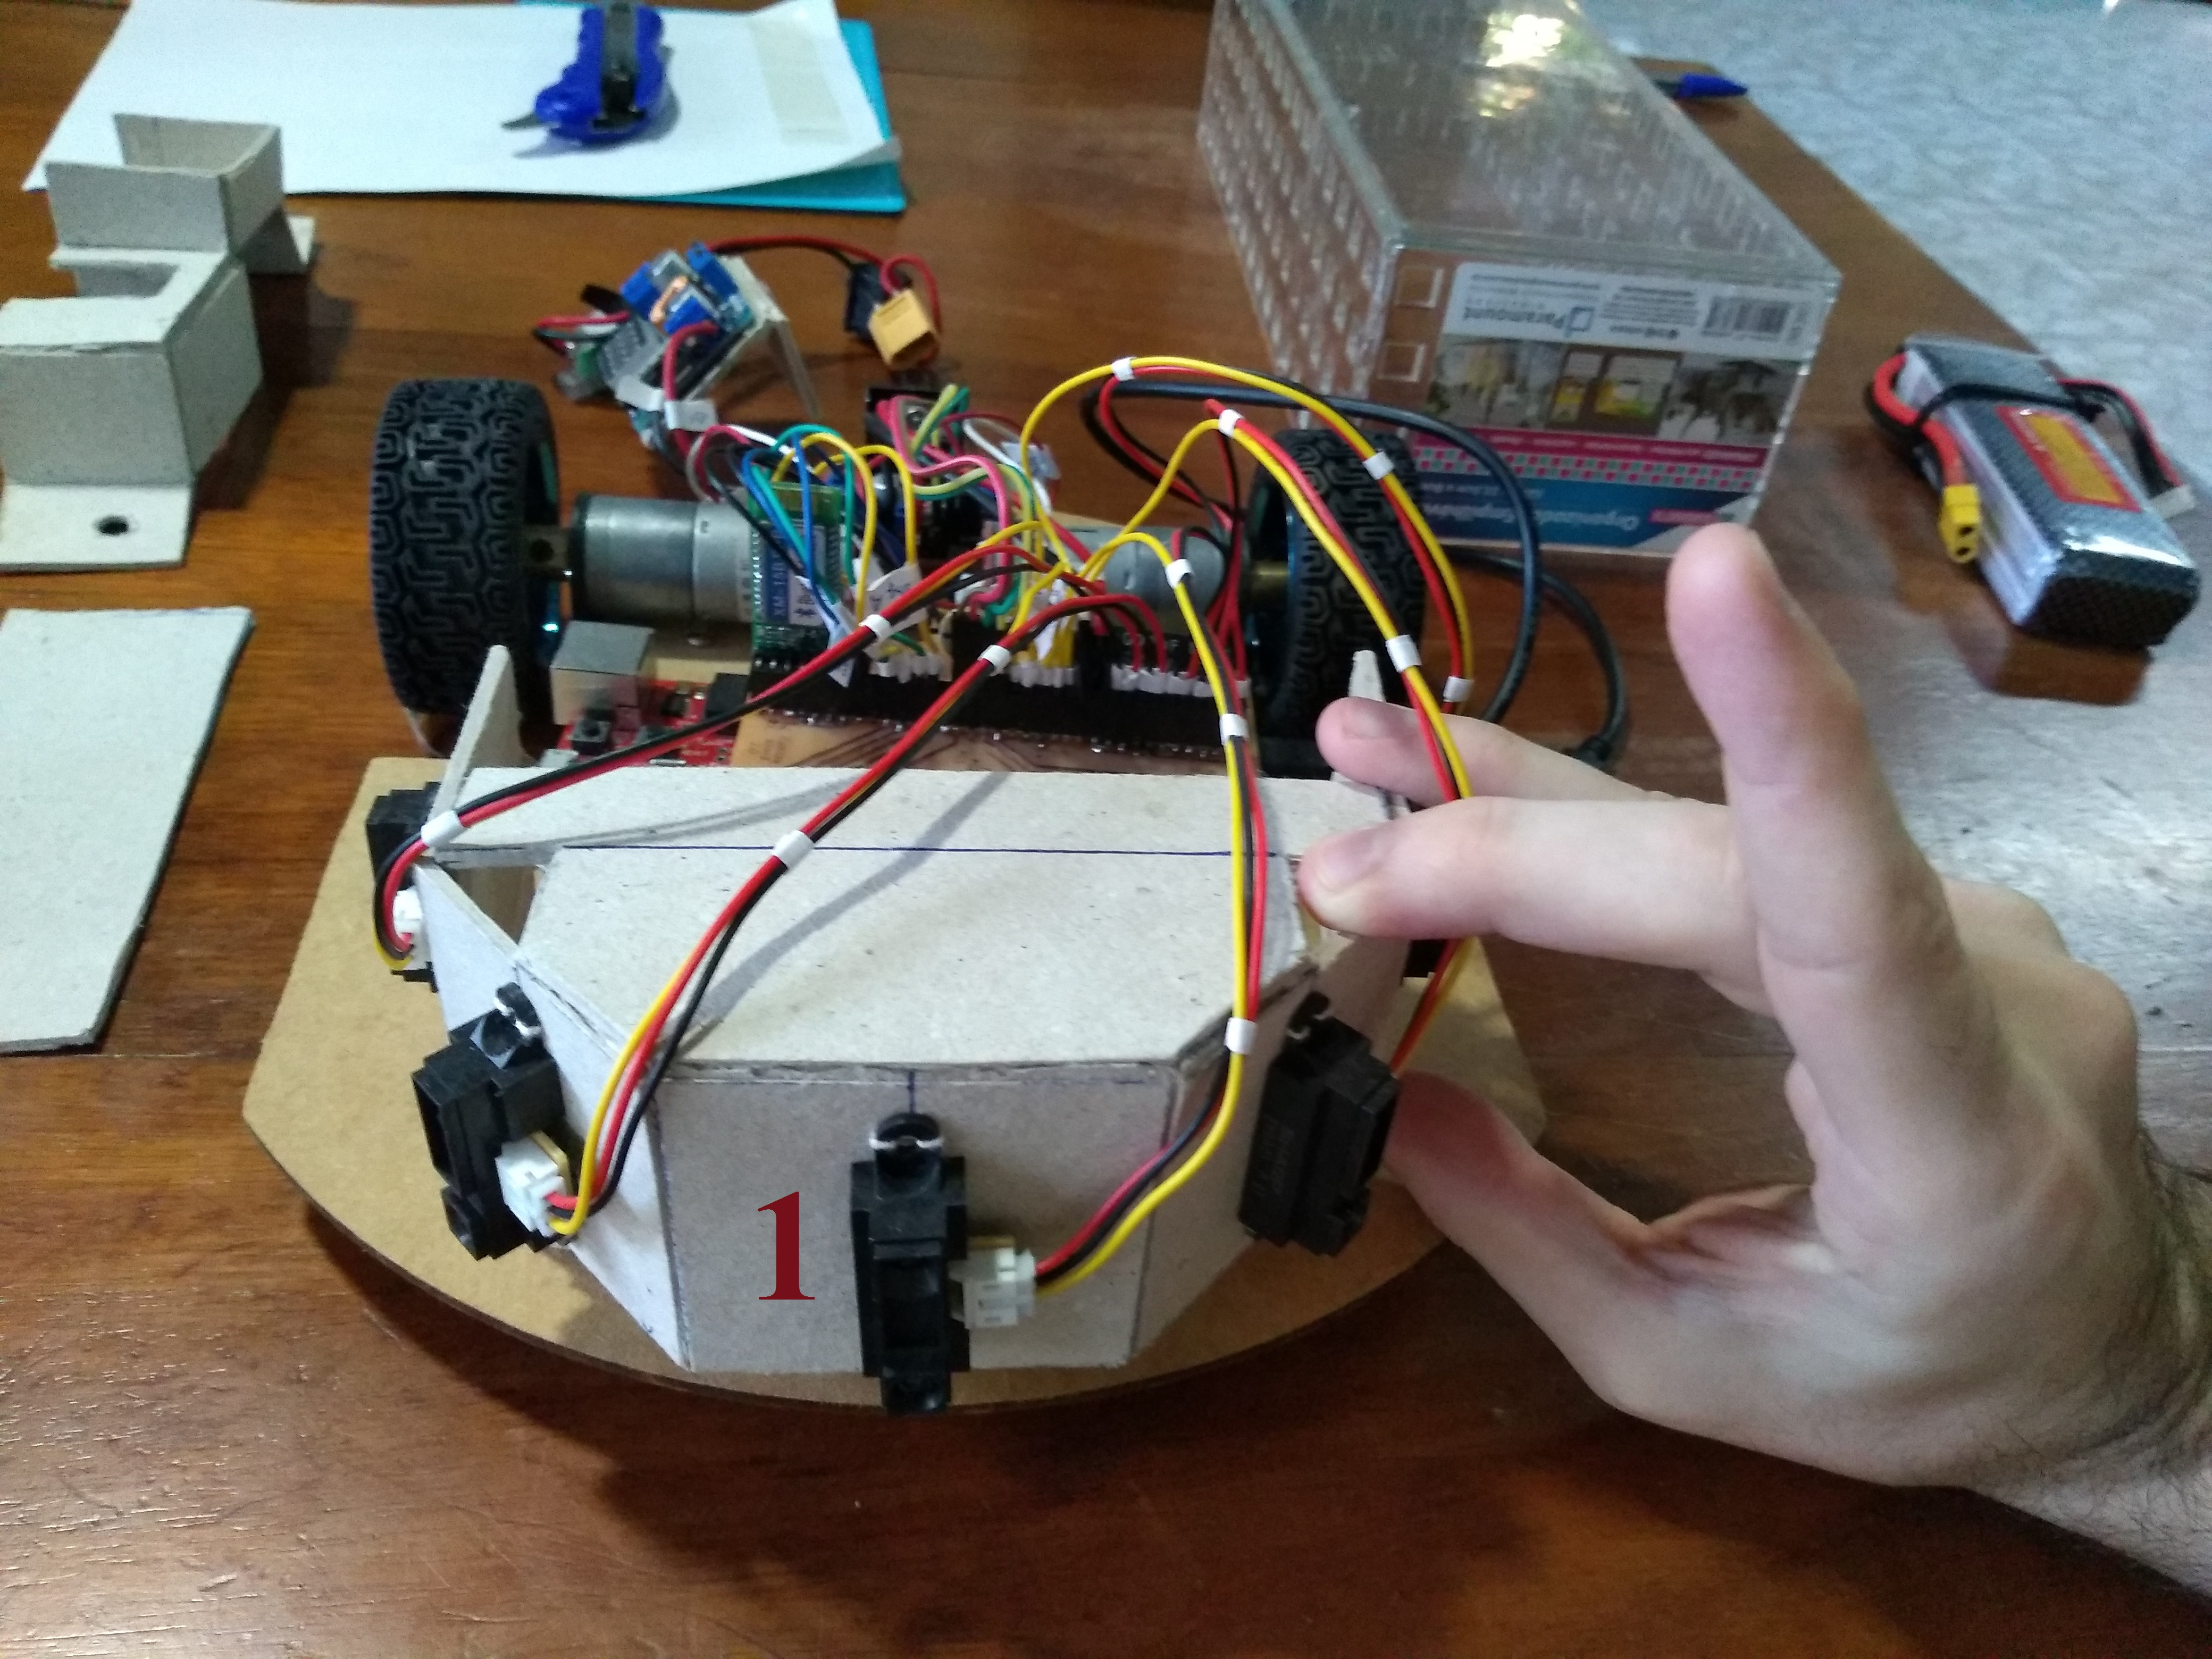
\includegraphics[trim= 0cm 0cm 0cm 0cm,clip,
scale=0.055]{Figuras/RoboMontagem1}
		\subcaption{Posicionamento dos sensores IR}
	  	%\label{fig:test1}
	\end{subfigure}
	~
	\begin{subfigure}[b]{0.49\textwidth}%
		\centering
		% fbox{}
		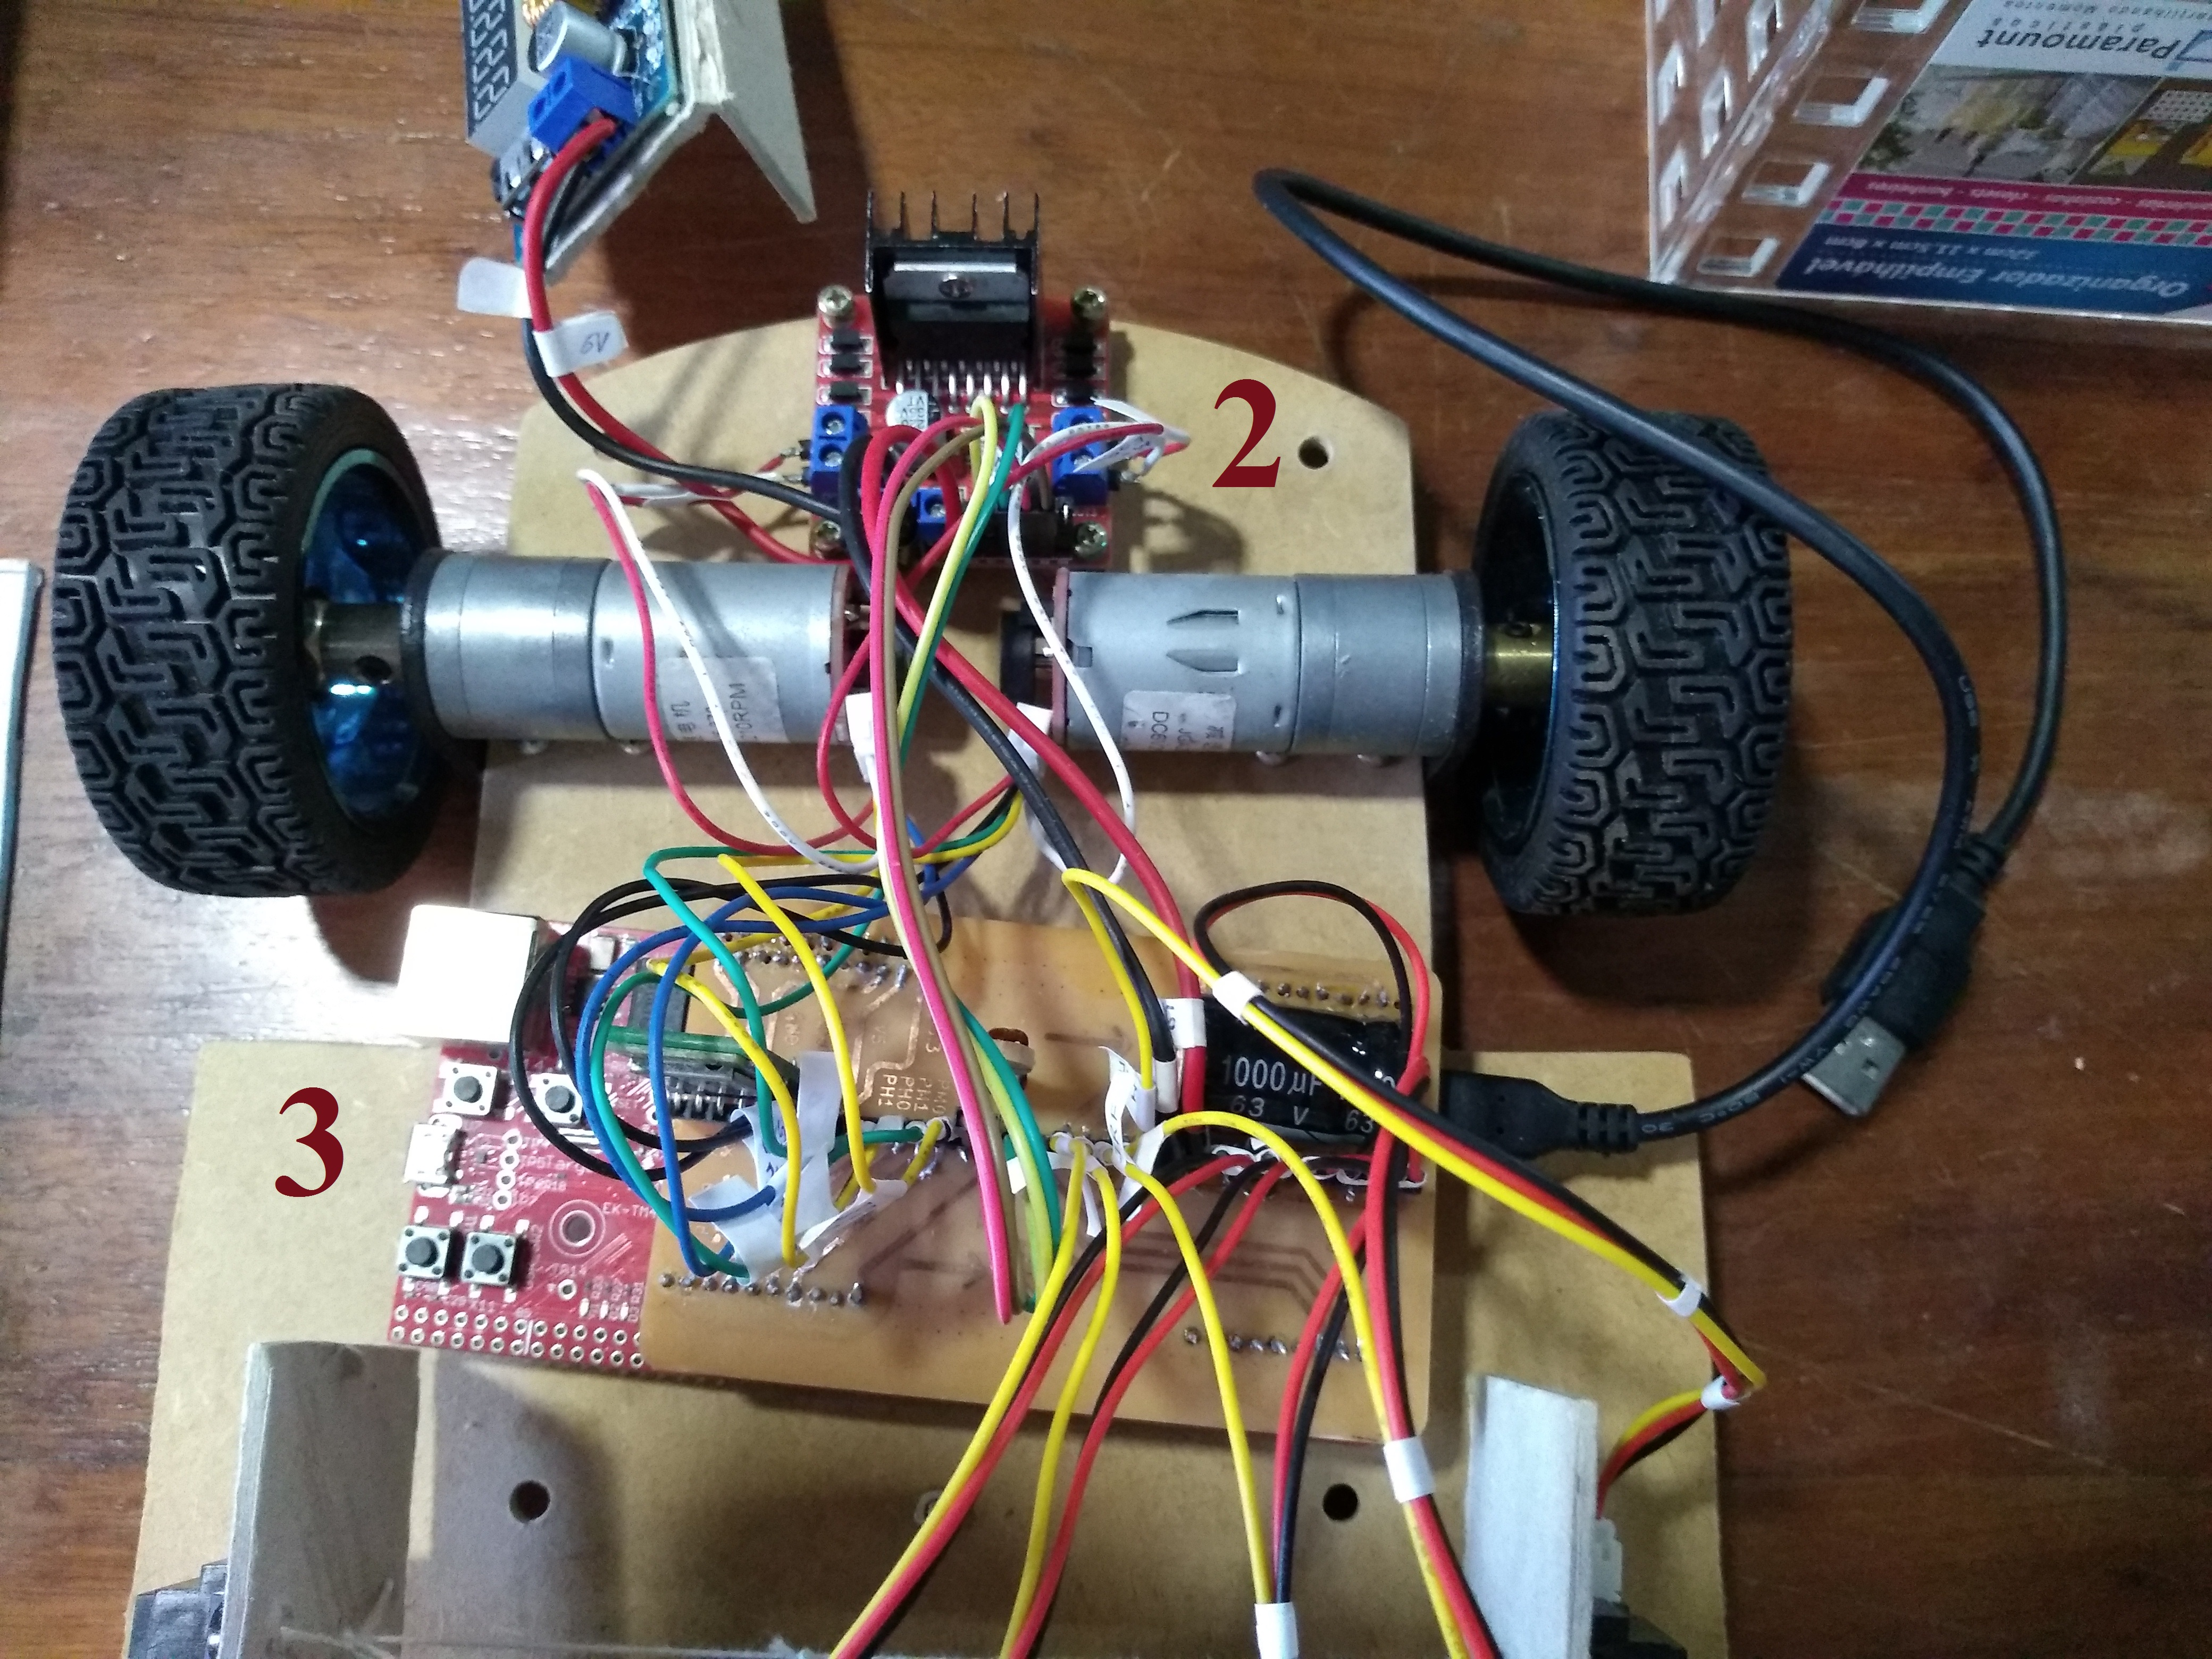
\includegraphics[trim={0cm 0cm 0cm 0cm},clip,
scale=0.055]{Figuras/RoboMontagem2}
		\subcaption{Disposição dos motores e microcontrolador}
	  	%\label{fig:test2}
	\end{subfigure}
	~
	\begin{subfigure}[b]{0.49\textwidth}%
		\centering
		% fbox{}
		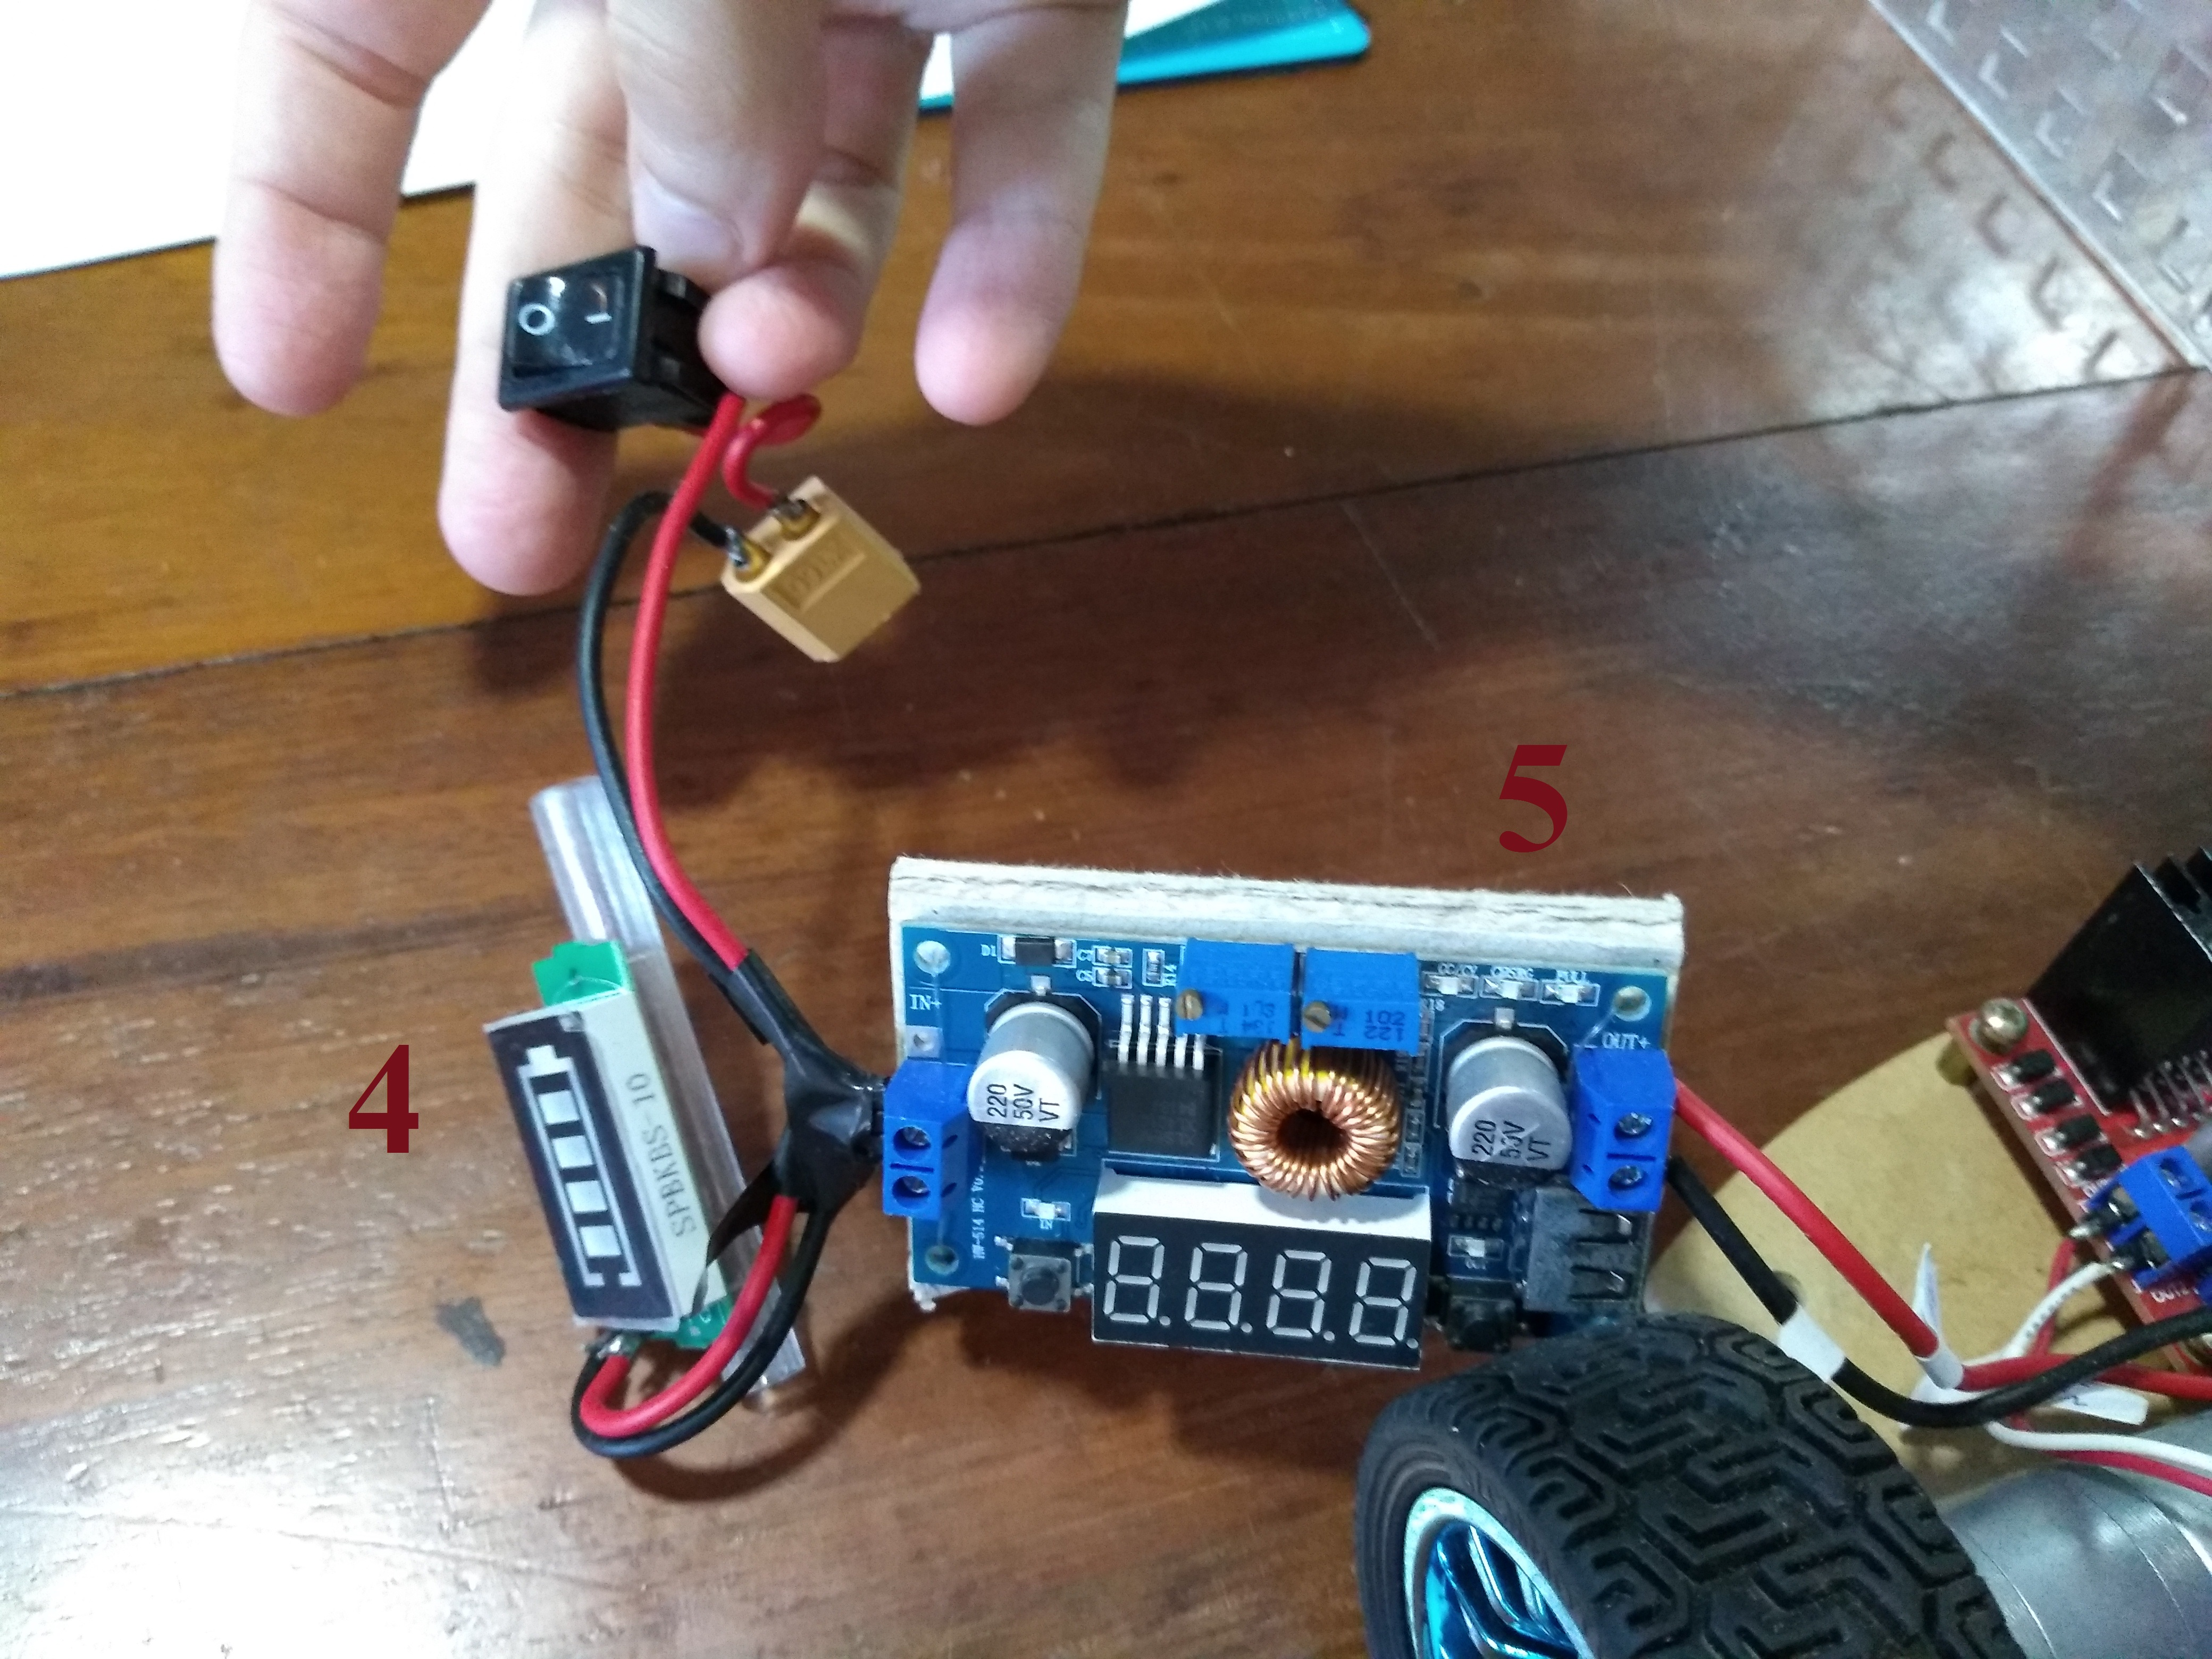
\includegraphics[trim= 0cm 0cm 0cm 0cm,clip,
scale=0.055]{Figuras/RoboMontagem3}
		\subcaption{Regulador de Tensão}
	  	%\label{fig:test1}
	\end{subfigure}
	~
	\begin{subfigure}[b]{0.49\textwidth}%
		\centering
		% fbox{}
		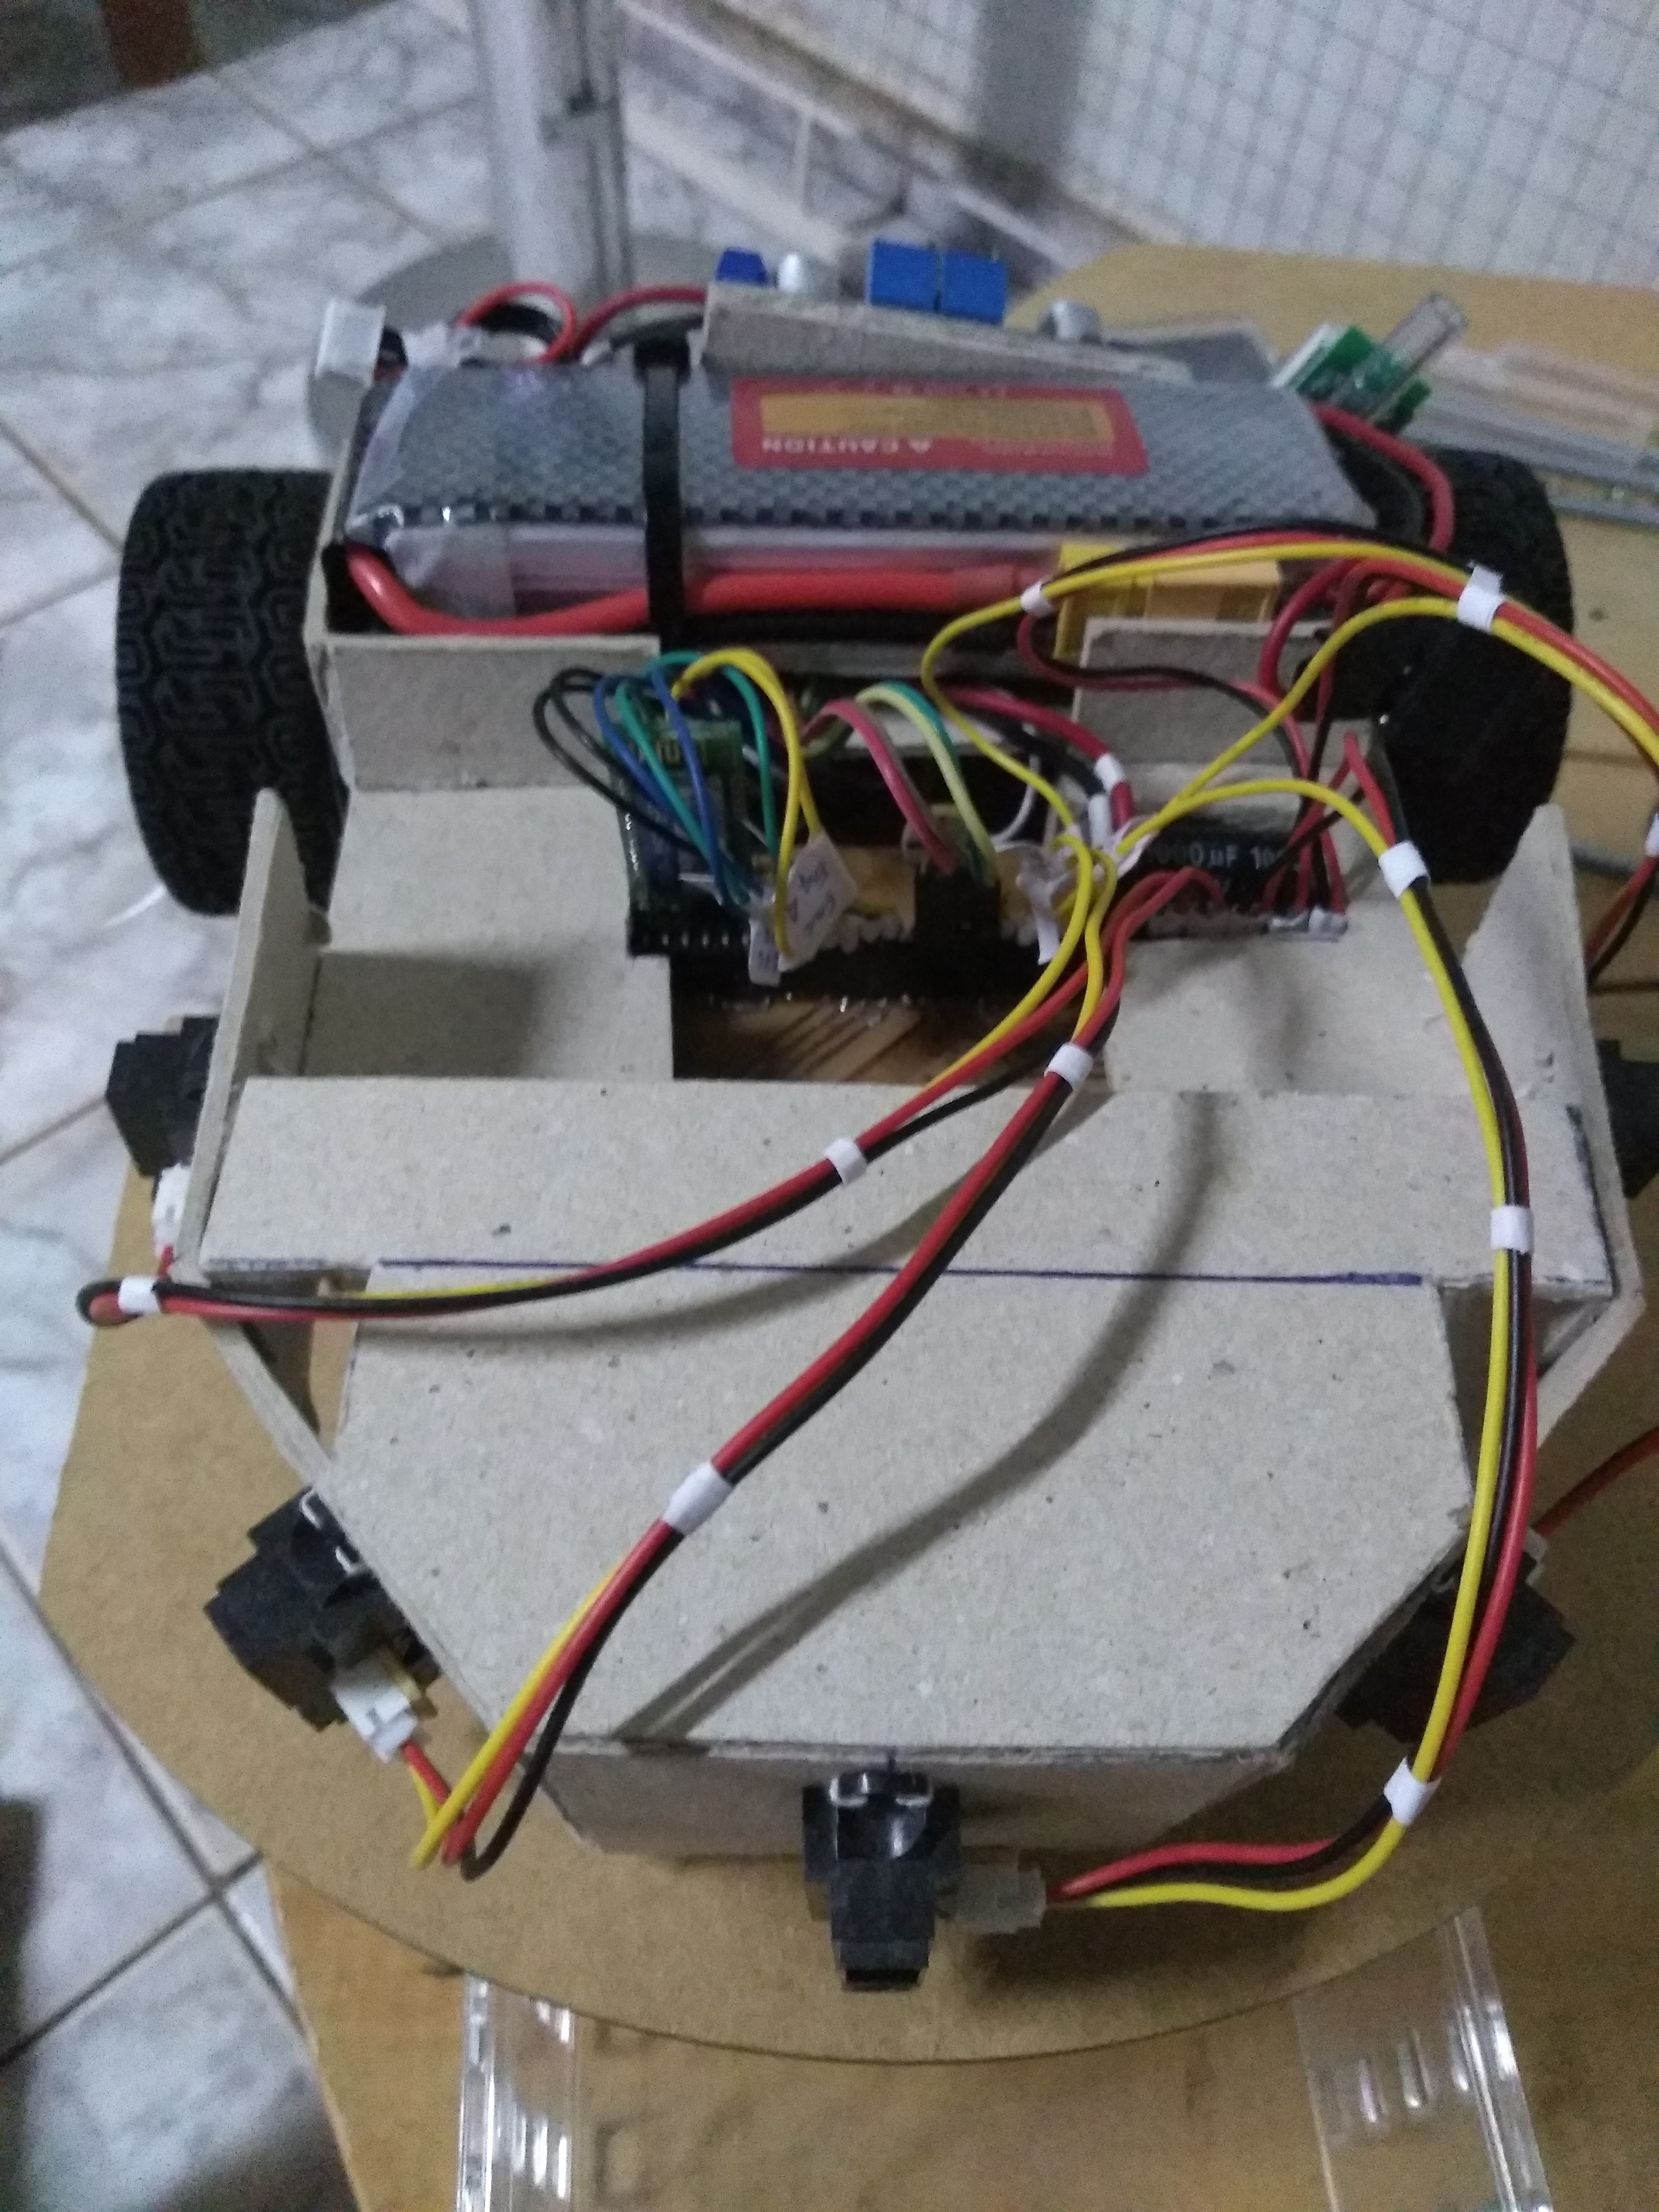
\includegraphics[trim={0cm 0cm 0cm 0cm},clip,
scale=0.055]{Figuras/RoboMontagem4}
		\subcaption{Posicionamento dos componentes}
	  	%\label{fig:test2}
	\end{subfigure}
	
	\textbf{Fonte: autoria própria}
\end{figure}
	
	O número 1 na Figura \ref{fig:RoboReal}.a indica o sensor infravermelho. Os números 2 e 3
	na Figura \ref{fig:RoboReal}.b indicam o driver e o microcontrolador, respectivamente.
	Os números 4 e 5 na Figura \ref{fig:RoboReal}.c indicam, respectivamente, o exibidor
	de nível energia para bateria de lítio (que não é necessário para o funcionamento) 
	e o regulador de tensão regulável. 
	
	A Figura \ref{fig:RoboReal2}.a mostra o posicionamento dos periféricos e parafusos 
	roscados. A Figura \ref{fig:RoboReal2}.b retrata a montagem concluída.
	
	\begin{figure}[!ht]
\centering
\caption{Robô após montagem}
\label{fig:RoboReal2}
	\begin{subfigure}[b]{0.49\textwidth}%
		\centering
		% fbox{}
		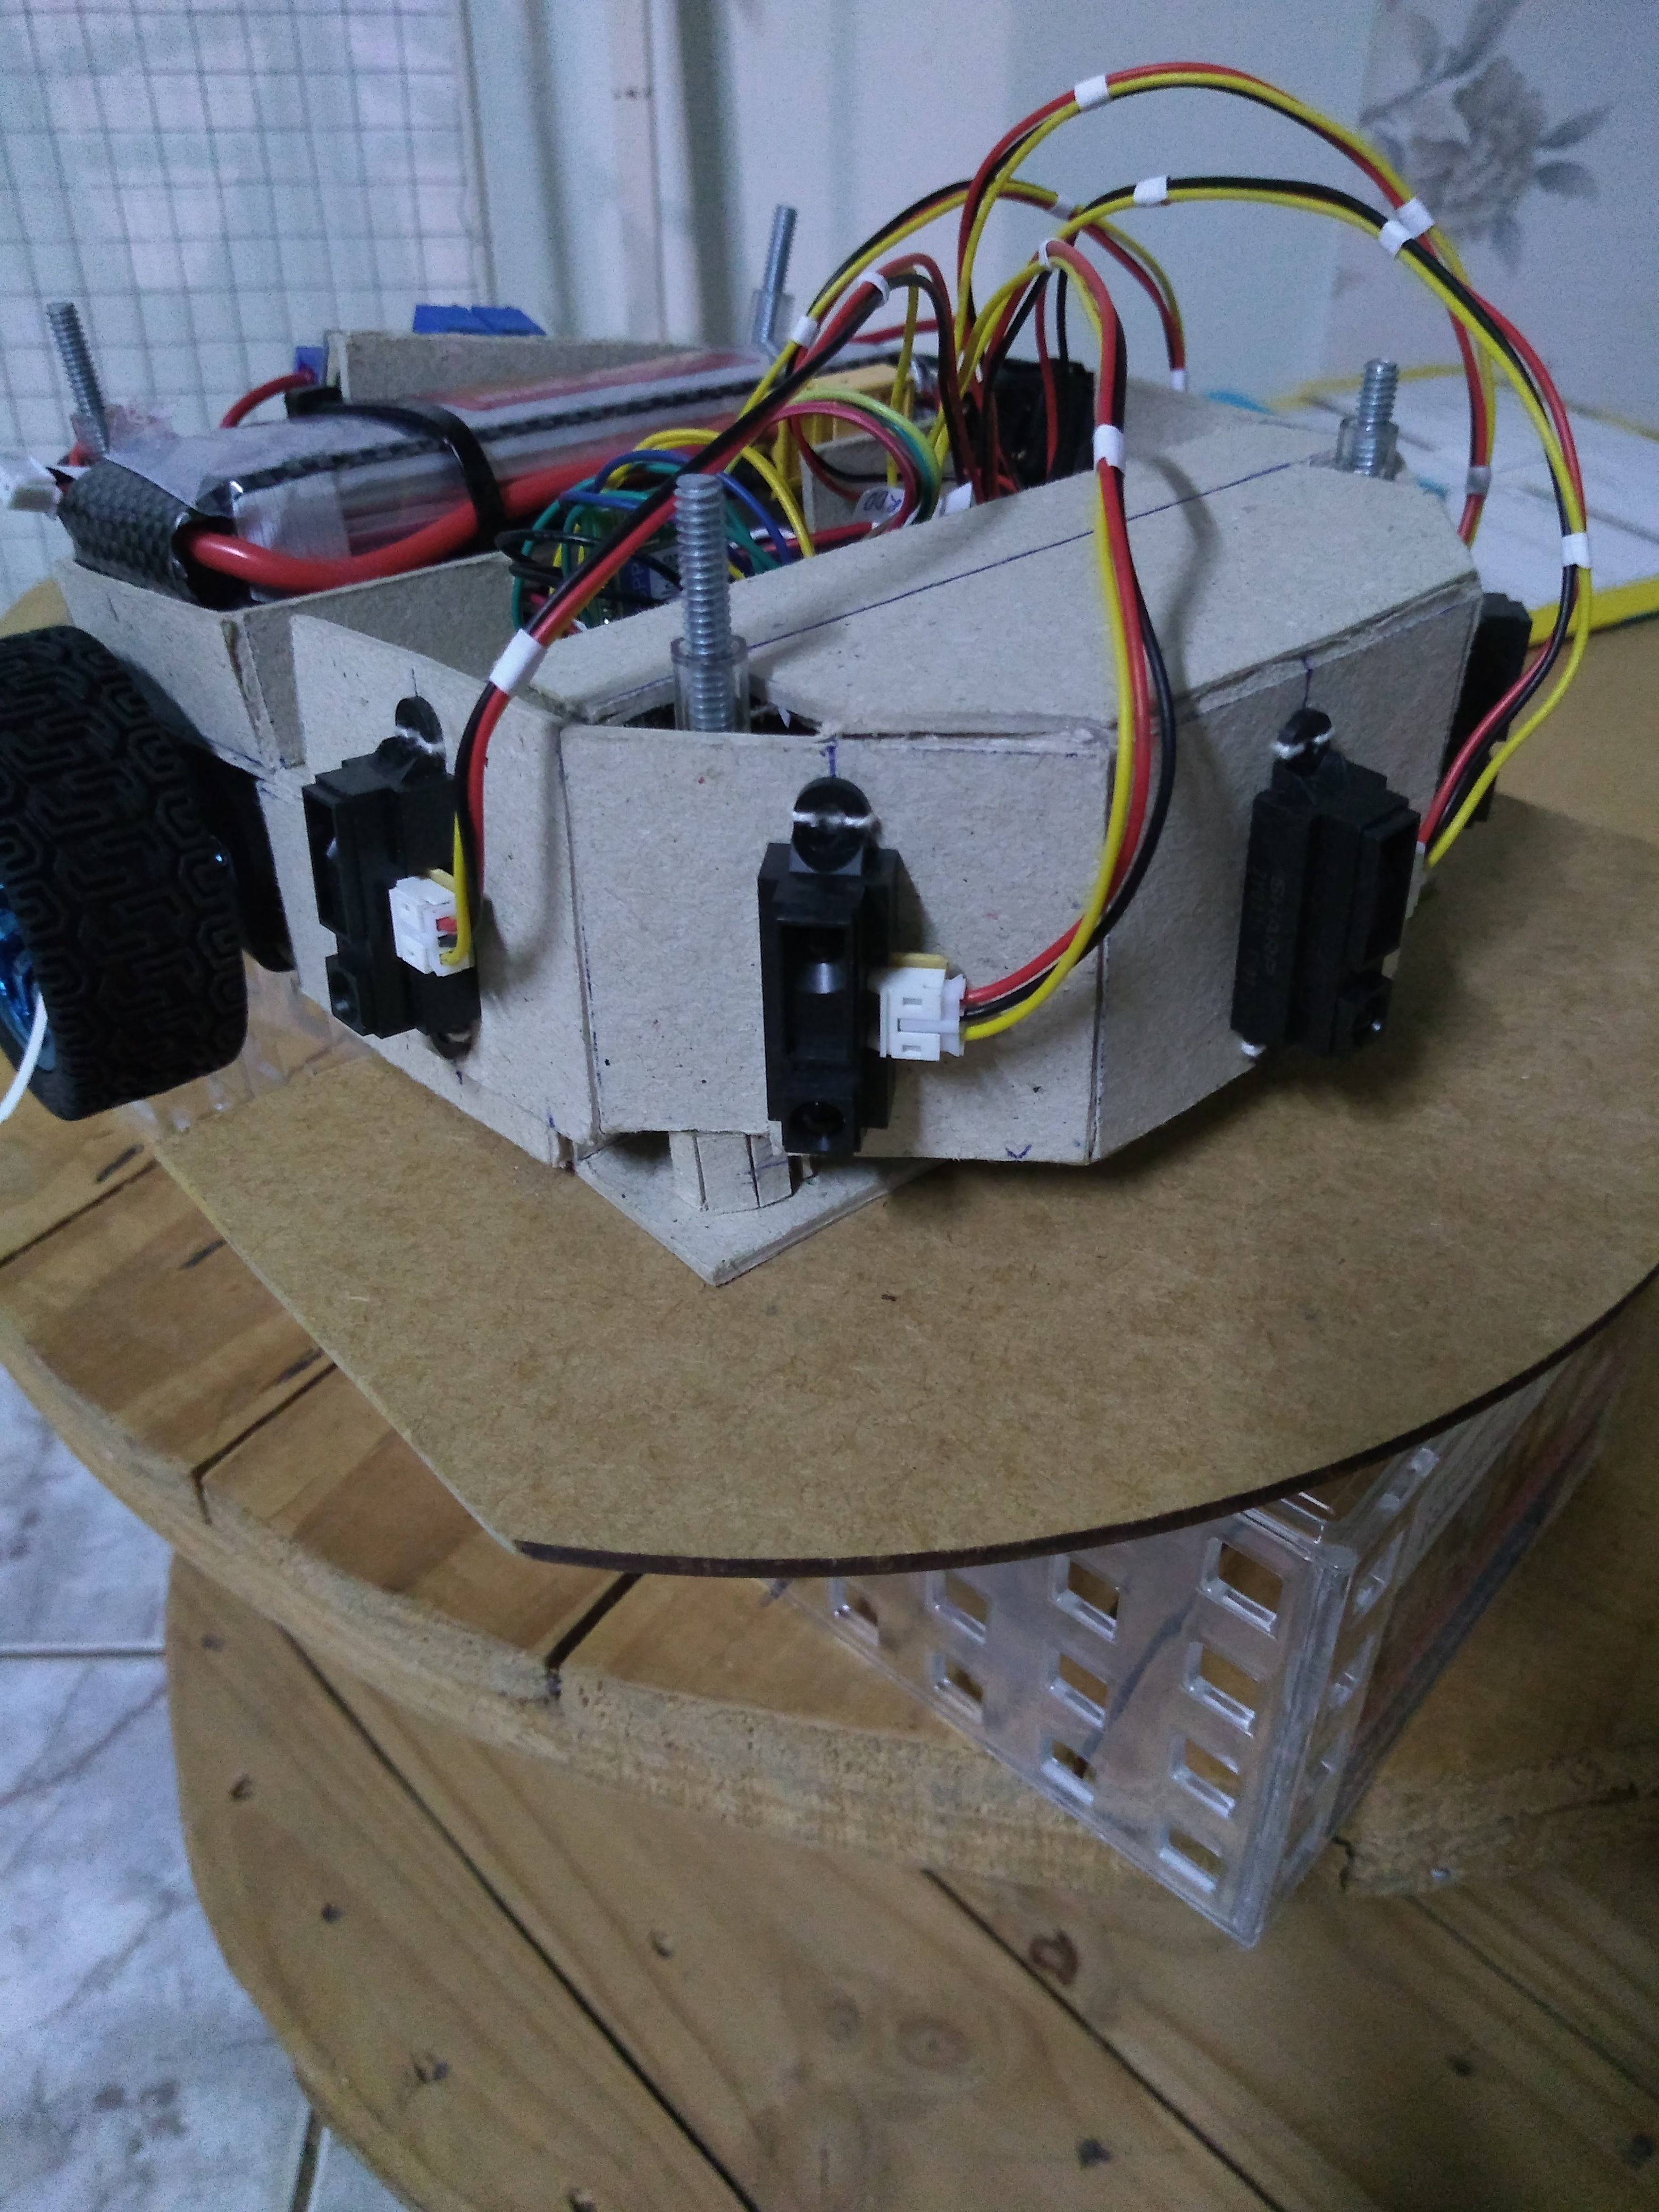
\includegraphics[trim={0cm 35cm 0cm 0cm}, clip, 
		scale=0.055]{Figuras/RoboMontagem5}
		\subcaption{Posição dos parafusos de rosca}
	  	%\label{fig:test1}
	\end{subfigure}
	~
	\begin{subfigure}[b]{0.49\textwidth}%
		\centering
		% fbox{}
		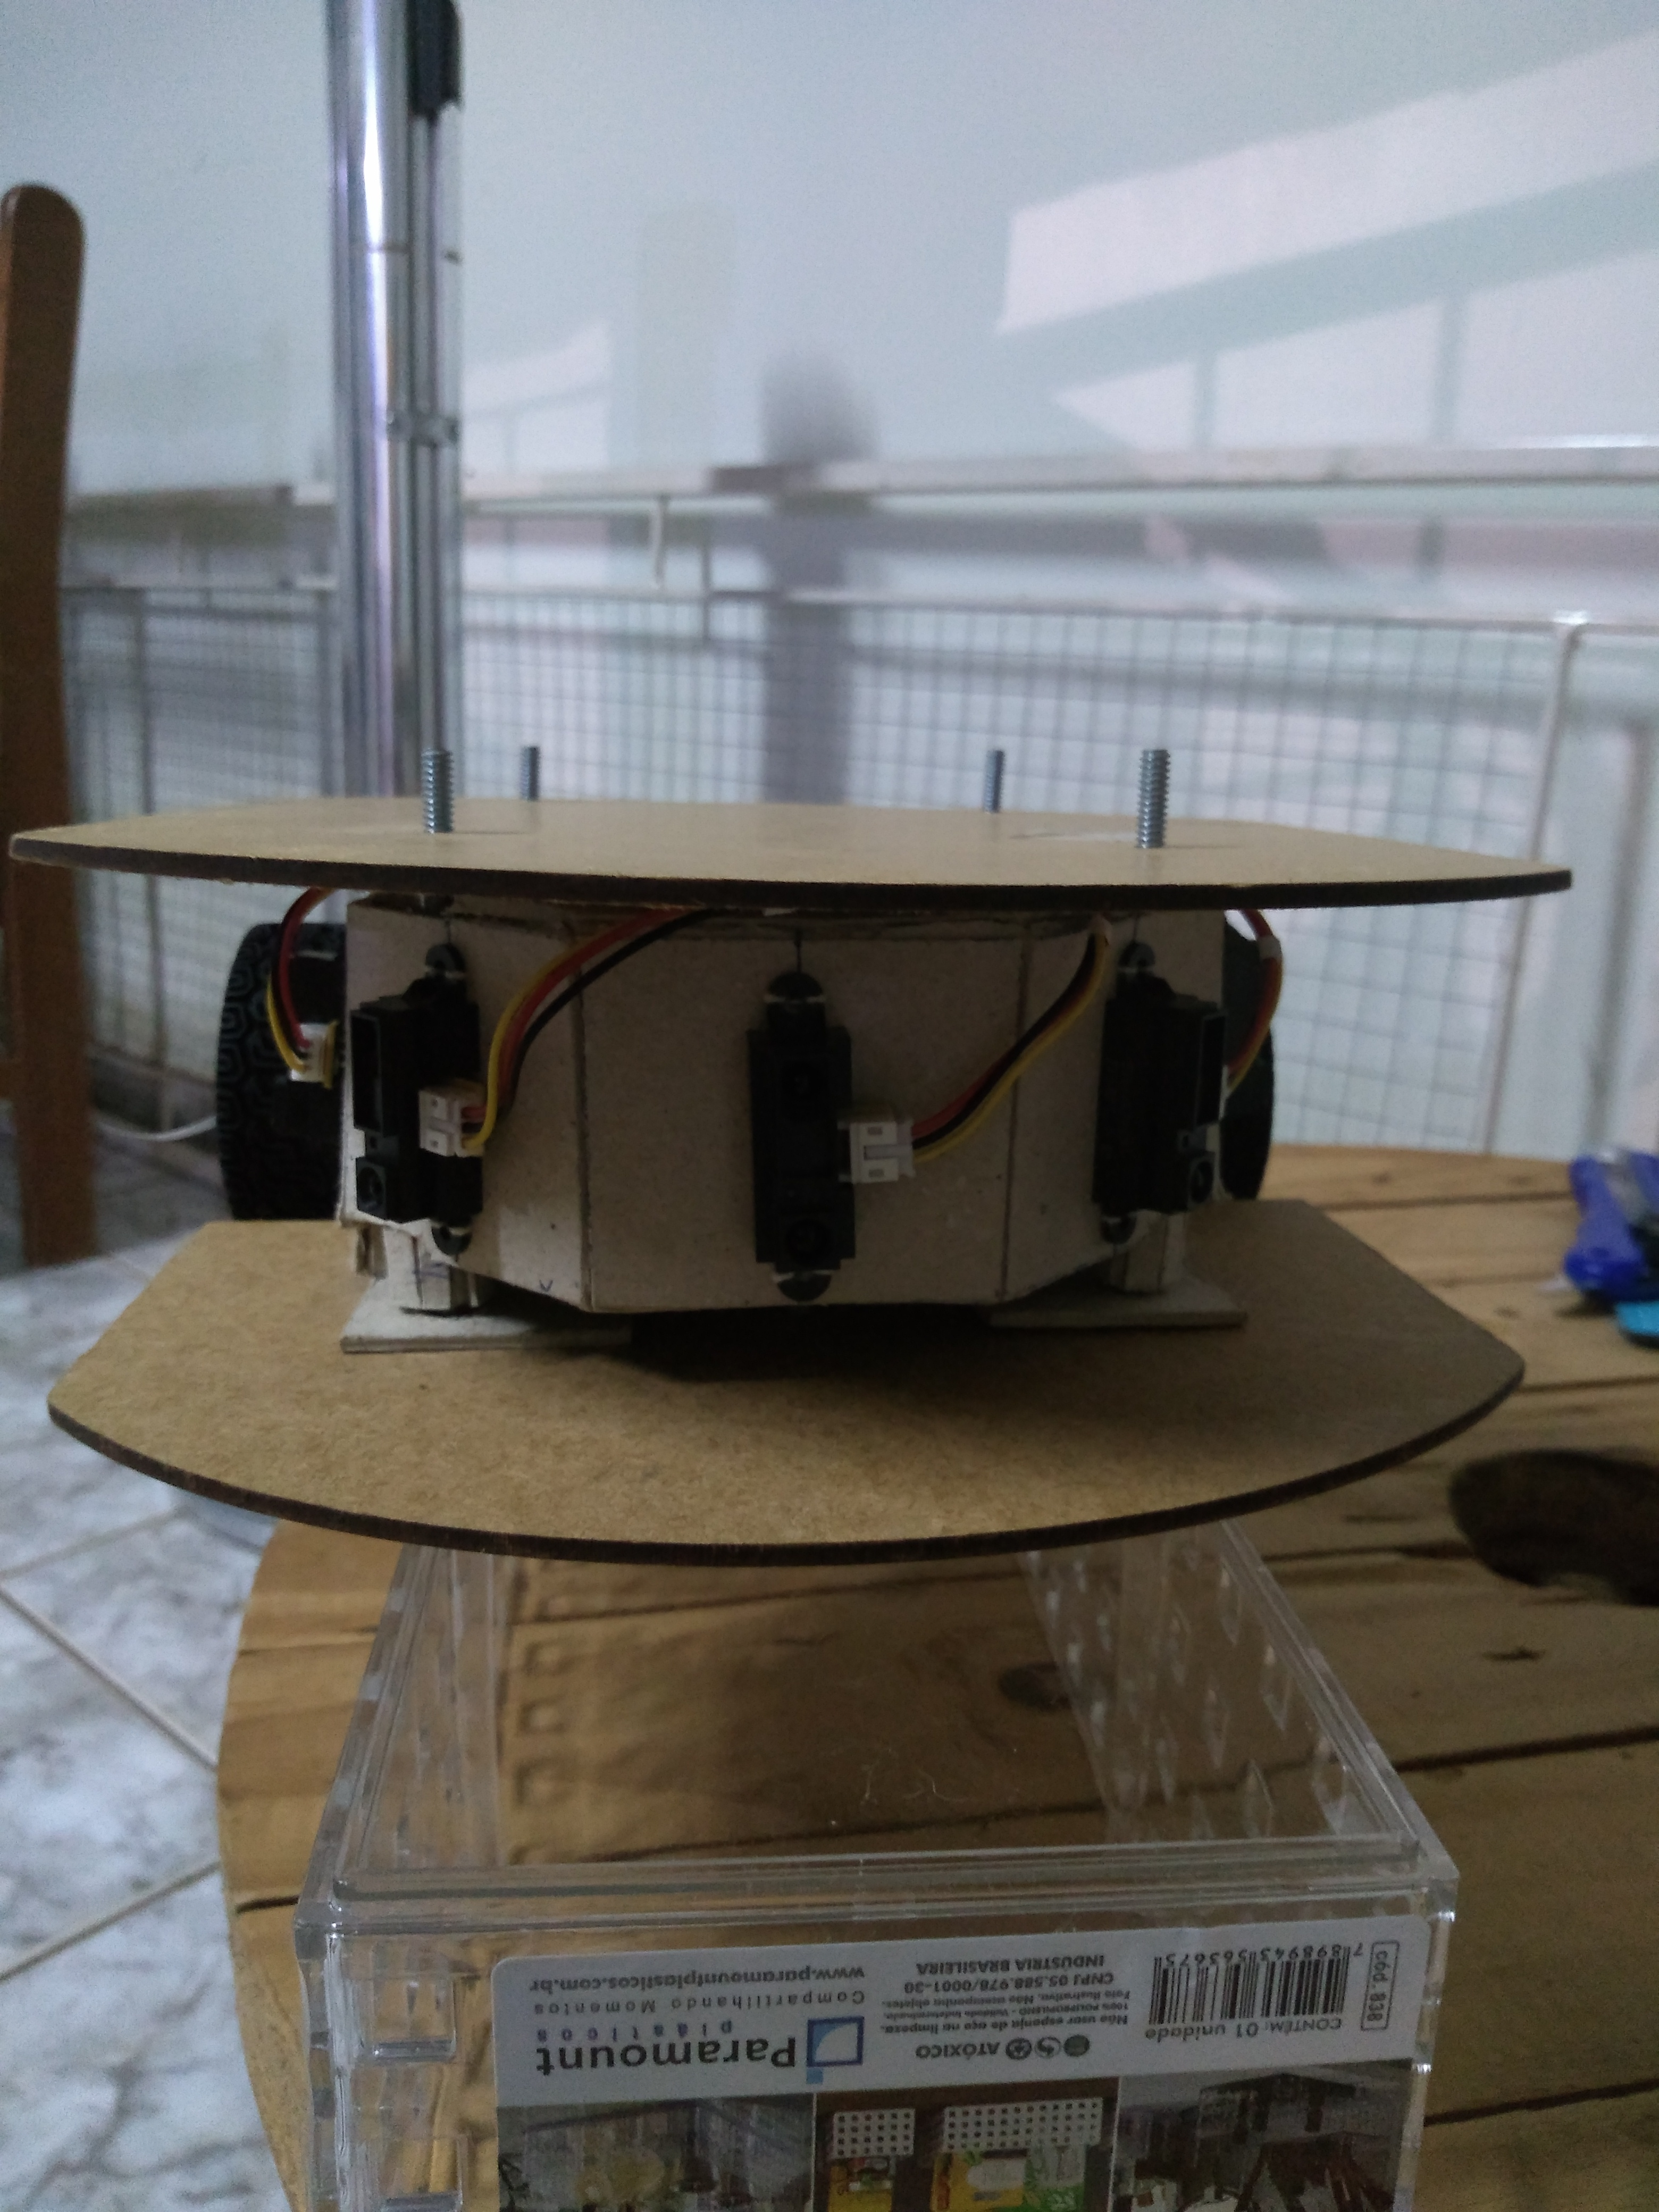
\includegraphics[trim={0cm 12.5cm 0cm 22.5cm}, clip, 
		scale=0.055]{Figuras/RoboMontagem6}
		\subcaption{Robô montado}
	  	%\label{fig:test2}
	\end{subfigure}
	\textbf{Fonte: autoria própria}
\end{figure}
	
\subsubsection{Curvas dos motores}

	A partir de um requisito de velocidade angular, é necessário definir a quantidade de 
	acionamento que será utilizada no motor (porcentagem de PWM).
	
	Para isso, foi feito um levantamento da curva dos motores. Ao alterar a porcentagem do
	acionamento PWM com incrementos de 1\%, a saída do sensor de efeito \textit{hall} é 
	utilizada para calcular a velocidade em rotações por segundo. 
	
	A Figura \ref{fig:acionamento1} mostra essa curva para o caso de ausência de carga, ou
	seja, o teste foi realizado sem que o pneu tocasse o chão. 
	
	\begin{figure}[!ht]
\centering
\caption{Curva do motor sem carga}
\label{fig:acionamento1}
		\centering
		% fbox{}
		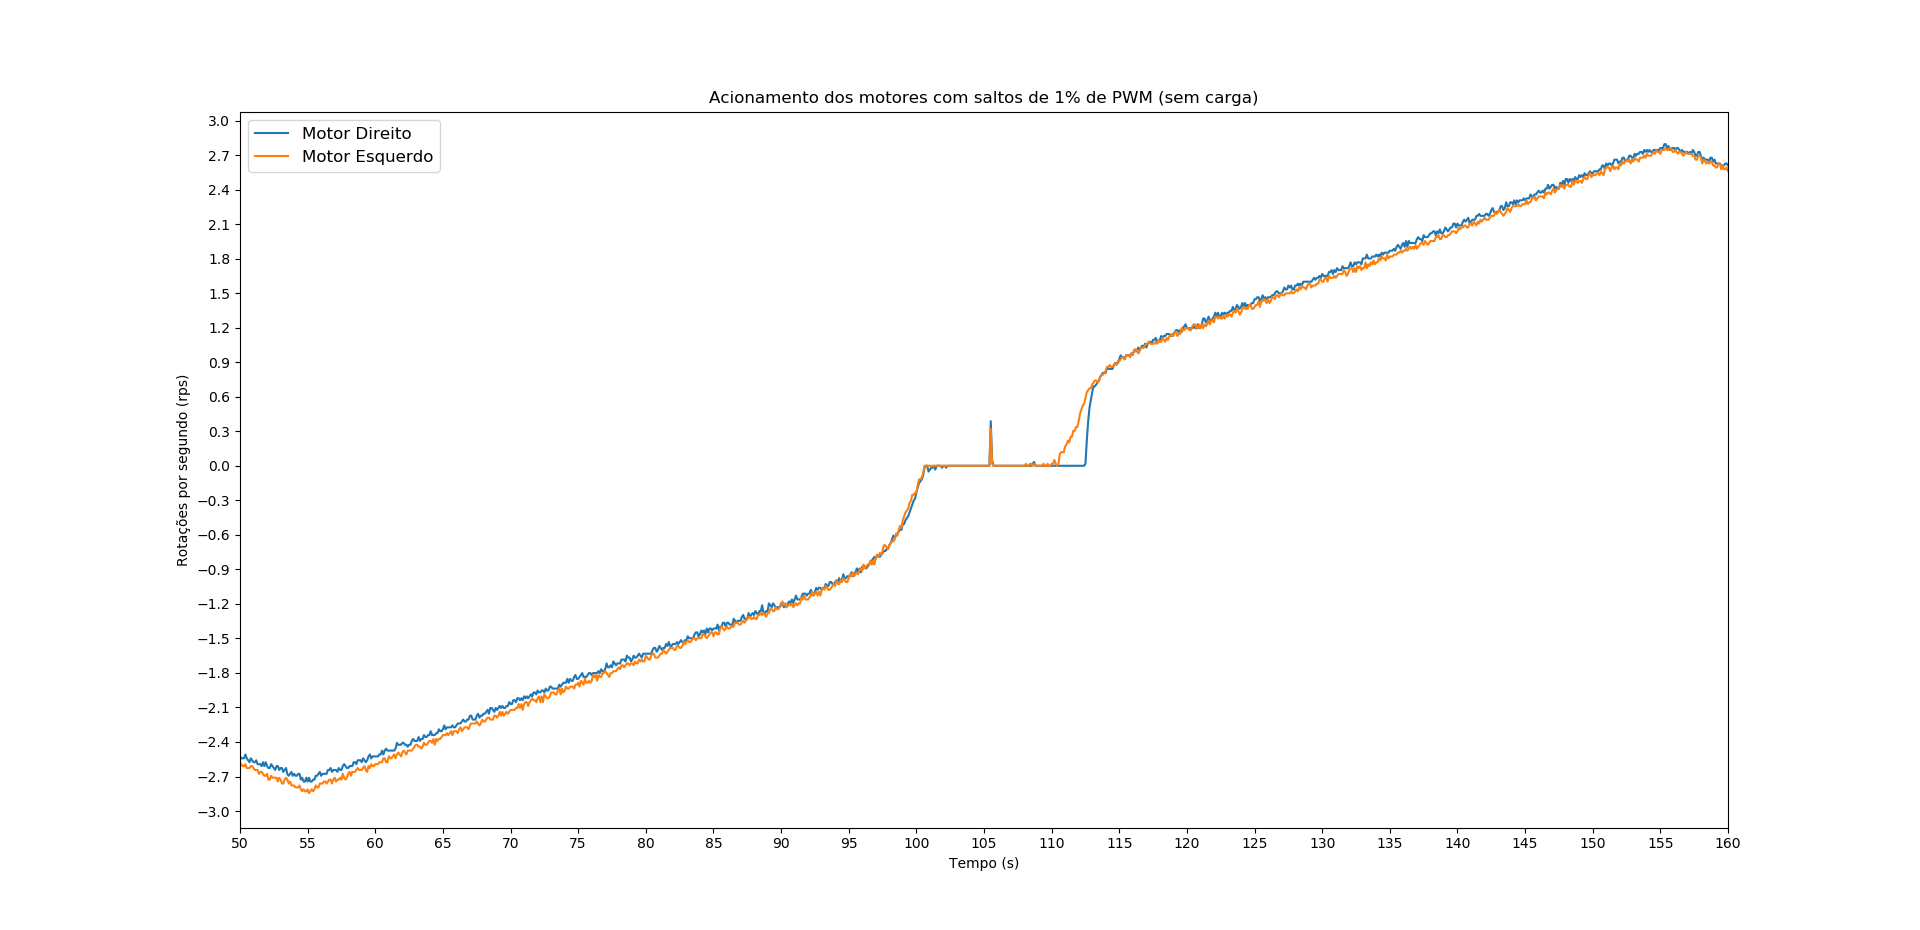
\includegraphics[trim={5cm 1cm 5cm 2cm},clip,
scale=0.38]{Figuras/Acionamento_Sem_Carga_rps}
	
	\textbf{Fonte: autoria própria}
\end{figure}
	
	A Figura \ref{fig:acionamento2} mostra a curva para o caso de presença de carga. Neste
	caso, o teste foi feito com o robô no chão, em uma quadra de esportes que, por não ter 
	o chão tão liso, levou a um gráfico bastante ruidoso. Os três pontos fora da curva 
	ocorreram devido a pequenos chutes dados no robô a fim de evitar uma colisão com parede.
	
	\begin{figure}[!ht]
\centering
\caption{Curva do motor com carga}
\label{fig:acionamento2}
		\centering
		% fbox{}
		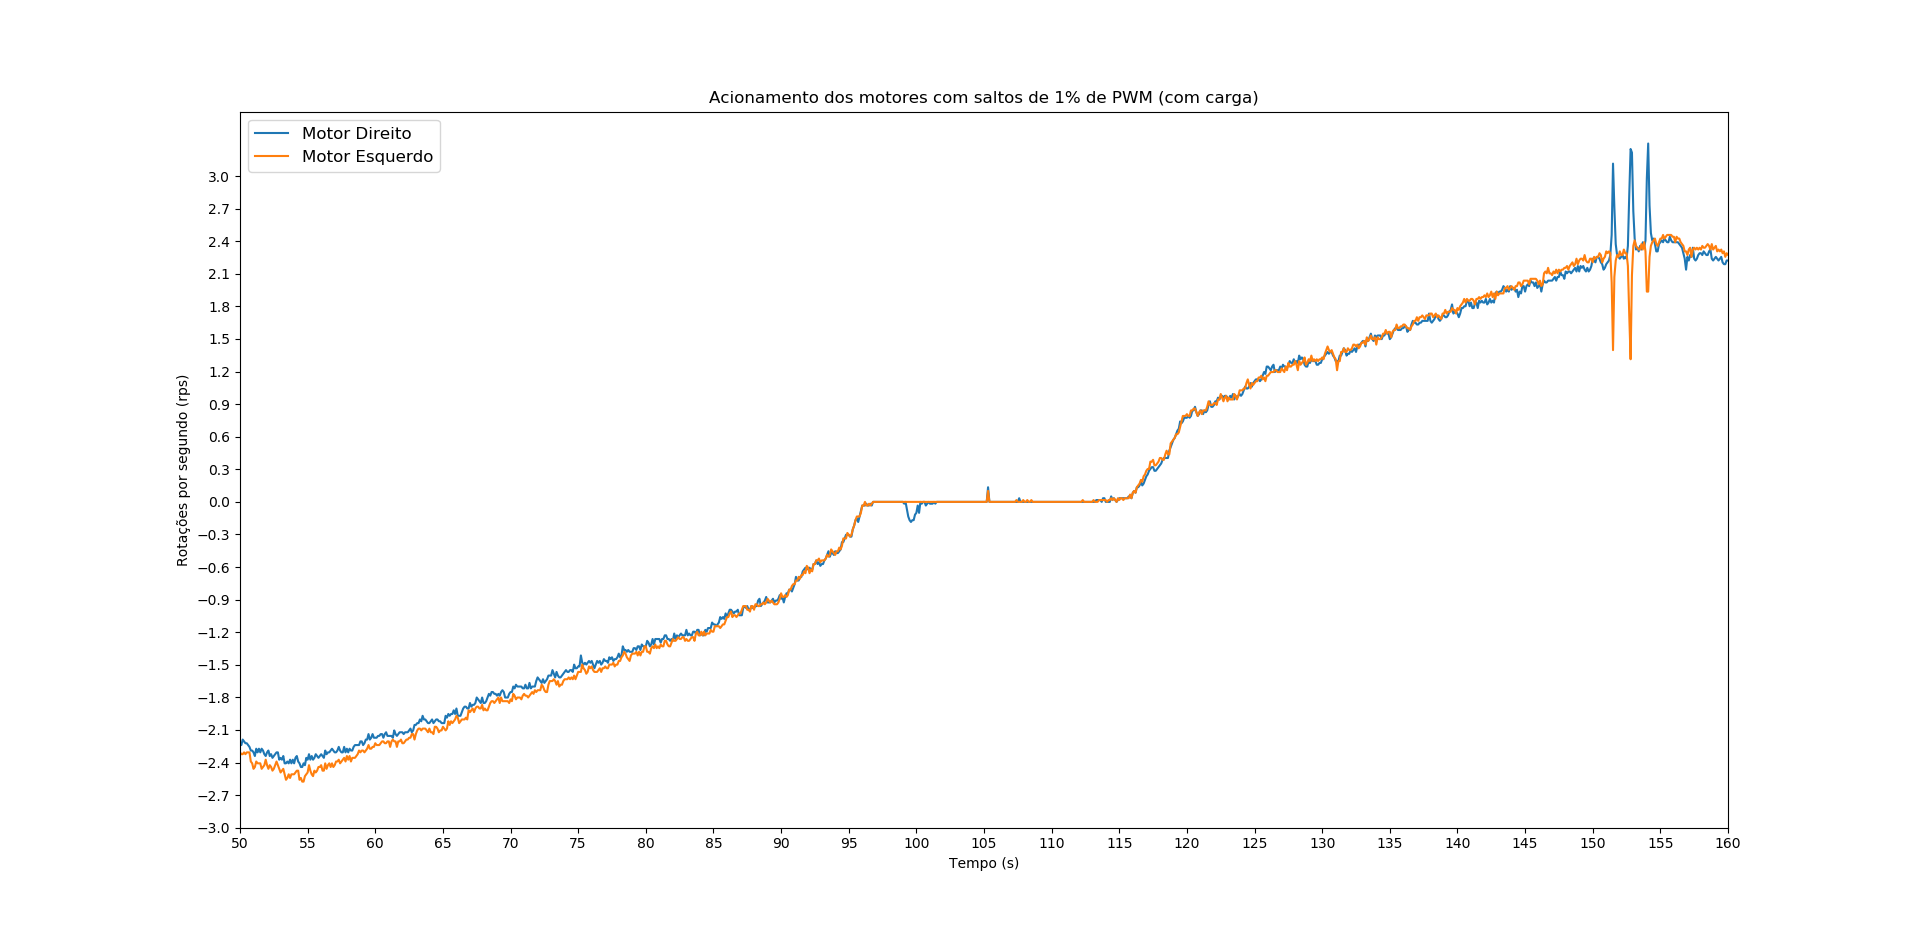
\includegraphics[trim={4.4cm 1cm 4.5cm 2cm},clip,
scale=0.38]{Figuras/Acionamento_Com_Carga_rps}
	
	\textbf{Fonte: autoria própria}
\end{figure}
	
	A partir do teste sem carga do motor direito, foi feita uma regressão linear utilizando 
	a parte da curva cujo regime é linear. A Figura \ref{fig:acionamento3} mostra o resultado 
	dessa regressão, bem como as constantes obtidas.
	
	\begin{figure}[!ht]
\centering
\caption{Regressão Linear para a curva do motor}
\label{fig:acionamento3}
		\centering
		% fbox{}
		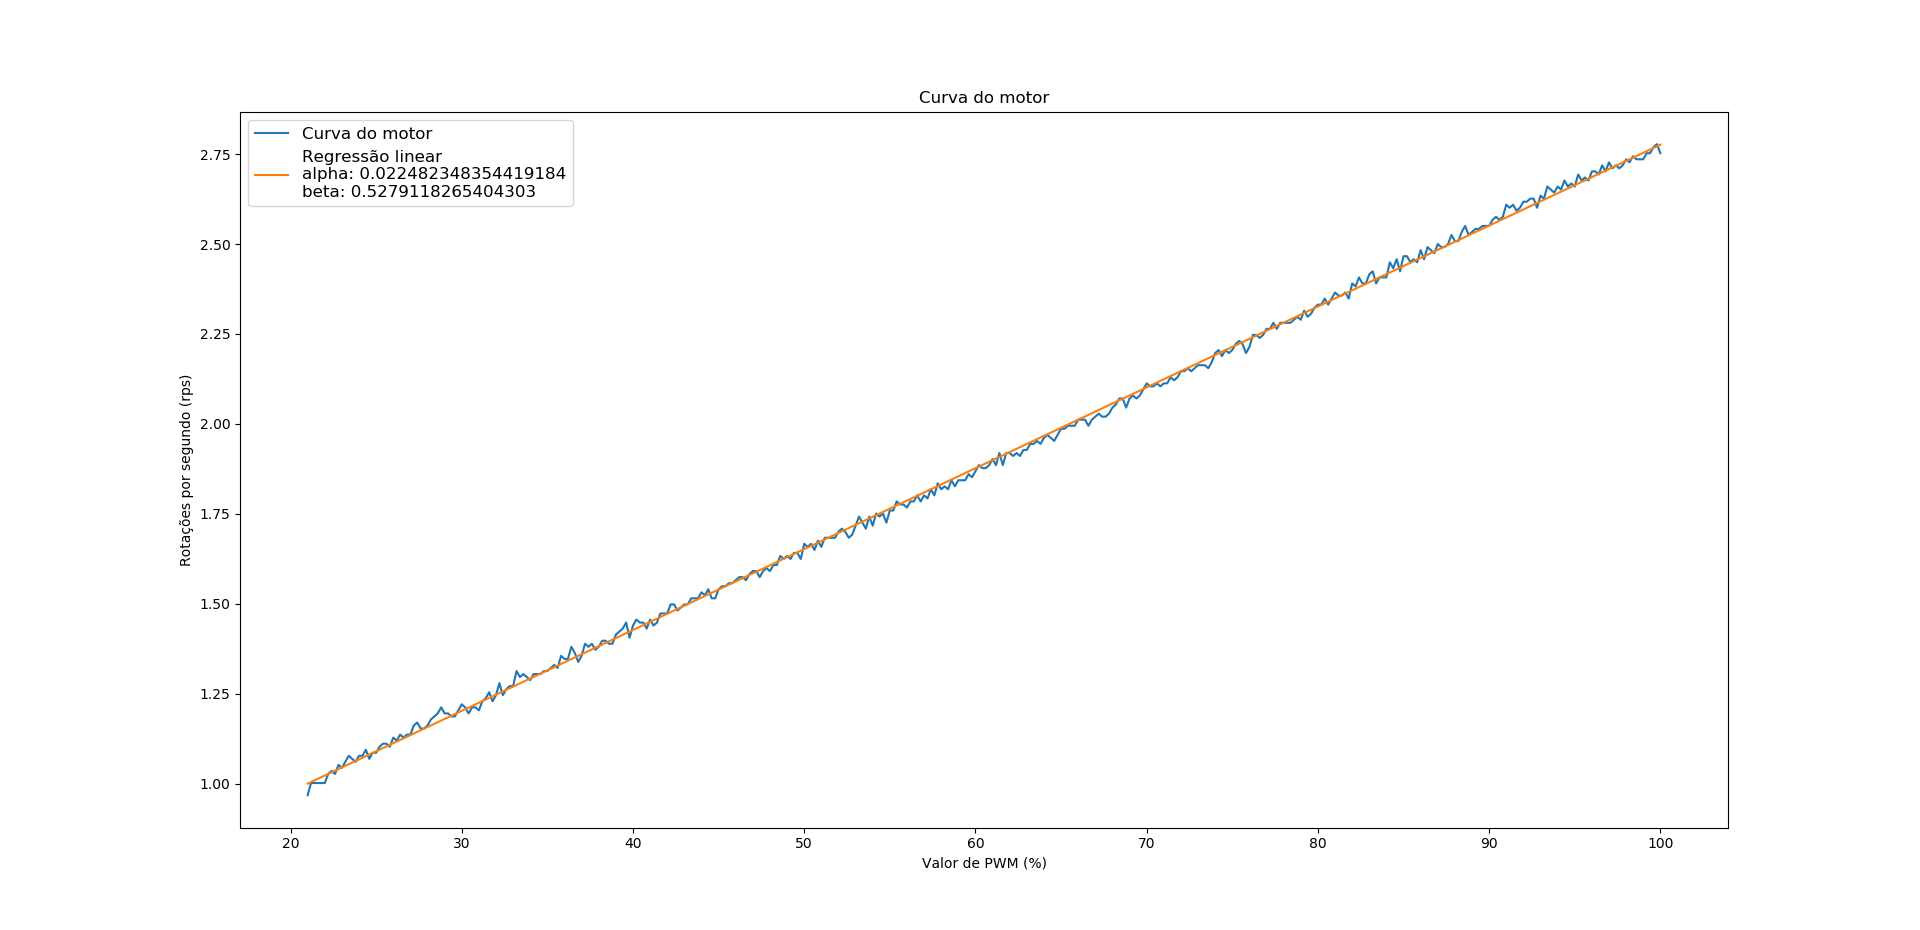
\includegraphics[trim={5cm 1cm 5cm 2cm},clip,
scale=0.38]{Figuras/Curva_Do_Motor_rps}
	
	\textbf{Fonte: autoria própria}
\end{figure}
	
\section{Metodologia}

Neste trabalho o protótipo será desenvolvido tendo como base o robô móvel de
acionamento diferencial Quickbot \cite{QuickBot}. Porém, esse robô se encontra
com alguns componentes de hardware obsoletos. Componentes mais atuais serão
utilizados.

O simulador Simiam será estudado de modo a permitir a inserção de novas
funcionalidades, como o módulo \textit{fuzzy}, pois este simulador foi
implementado visando a utilização de uma arquitetura de controle híbrida (SED em conjunto
com SDVC). 

Em seguida, deve-se projetar os comportamentos do robô que solucionem o problema
proposto de duas maneiras separadas: utilizando o sistema híbrido, a fim de estudar a
estratégia de arbitragem de comportamentos, e por sistema \textit{fuzzy}, a fim de compreender 
a estratégia de fusão de comportamentos. 

Utilizar o simulador Simiam, desenvolvido pela Universidade Georgia
Tech, para validar o algoritmo de controle.

Deve-se executar a montagem física, implementar o sistema embarcado e elaborar os testes em
protótipo, utilizando obstáculos em posições distintas a fim de verificar a robustez dos 
algoritmos implementados. 